\status{started}
\chapter{MEG II and the Cockcroft–Walton}
\label{ch:MEG}
\begin{refsection}
{\itshape This Chapter is dedicated to an in-depth description of the MEG II search and apparatus. After the description of the different subdetectors and their functionality a description of the beamlines will follow. MEG II is served by the main muon beamline, part of the PSI beamlines described in the Introduction Chapter, and a secondary proton beamline equipped with its own Cockcroft–Walton. This machine has different uses in the collaboration, which will be here discussed, and its functioning has been one of my main tasks. For this reason, some additional details will be here included. Most of the information on MEG II can be found in the two recent papers: detector \cite{MEG_II:detector} and 2021 data-analysis \cite{MEG_II:2021}.}

\status{review}
\section{MEG II}
    The MEG II experiments aims at improving the limit set by its predecessor: $BR(\Am\ra\Ae\upgamma)<\num{4.2e-13}$ \cite{MEG} down to $\sim\num{6e-14}$.
    The signature of this process is a back-to-back pair of $\g$ and $\Ae$, with $E_\g = E_{\Ae} = \SI{53.2}{MeV}$.
    The main background is the accidental coincidence of high momentum positrons from Michel decay $\Am \ra \Ae \upnu_e \bar{\upnu}_\upmu$ and high energy photons from the radiative muon decay (RMD) $\Am\ra\Ae\upnu_e \bar{\upnu}_\upmu\g$, positron Bremsstrahlung or positron annihilation.\\
    The experiment, which is located at PSI, is currently running and a sketch of it is shown in Fig.~\ref{fig:MEGII}
    In particular, the muons are delivered by the $\uppi E5$ beamline.
    The key aspects of the upgrade are: a thinner and more slanted target, a pixelated Timing Counter (pTC), a new Cylindrical Drift CHamber (CDCH), the addition of a Radiative Decay Counter, a finer granularity for the Liquid Xenon Calorimeter (XEC) using MPPC, new electronics and calibration methods.
    The kinematic variables associated with the positron are measured with the spectrometer (COnstant Bending RAdius magnet (COBRA)+CDCH+pTC). 
    The kinematic variables (E, t, position) of the $\g$, expected to be monochromatic at $52.8$ MeV, are measured with the XEC.
    This is a 1000 $\ell$ ``c-shaped'' Liquid Xe calorimeter, equipped with both PMT and SiPM.\\
    \paragraph{Coordinate system}
    The coordinate system used is cylindrical $(r, \phi, z)$ with its origin located at the center of COBRA. 
    The $z$-axis aligns with the COBRA axis, coinciding with the direction of the incoming muon beam. 
    The azimuthal angle $\phi = 0$ is positioned opposite the center of the LXe detector and corresponds to the $x$-axis, with the $y$-axis pointing upwards. 
    Positrons follow trajectories characterized by decreasing $\phi$ coordinates. The polar angle $\theta$, measured with respect to the $z$-axis, is also employed. 
    The region where $z < 0$ is referred to as upstream, while the region where $z > 0$ is termed downstream.
    The size of the LXe fiducial volume defines the geometrical acceptance of $\sim 11\%$: $\phi_\gamma \in [\frac{2}{3}\pi, \frac{4}{3}\pi]$ and $|\cos\theta_\gamma| < 0.35$. 

    \begin{figure}
        \centering
        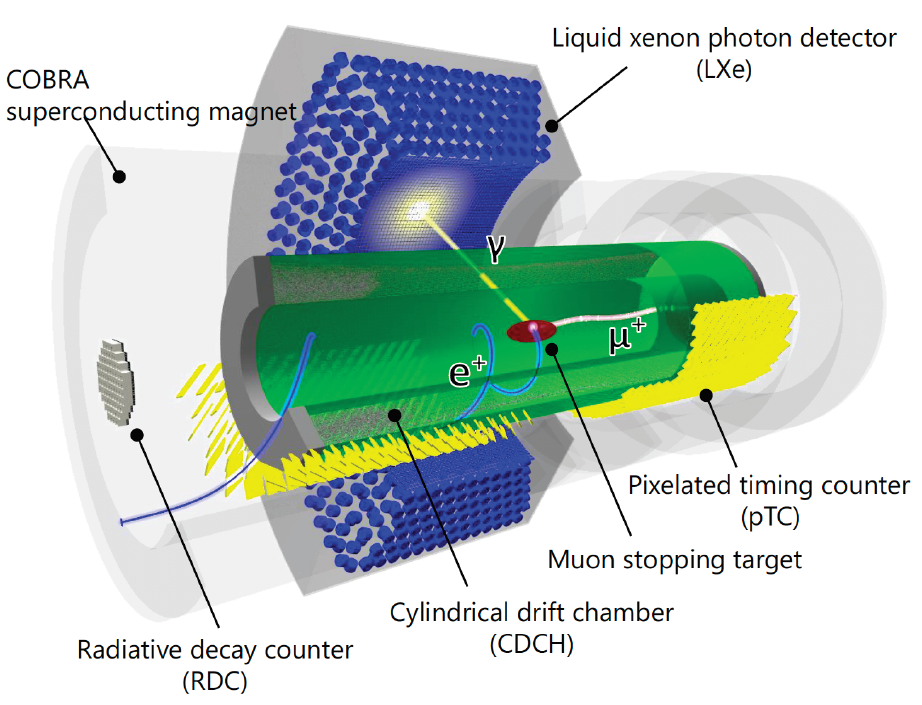
\includegraphics[width = 0.8\textwidth]{Figures/Introduction/MEG_II.png}
        \caption{Sketch of the MEG II apparatus with a $\Am\ra\Ae\g$ event.}
        \label{fig:MEGII}
    \end{figure}

    \paragraph{Alignment} The analysis of the relative alignment within each detector, like the extraction of the \textit{real} position of the wires in the CDCH, and between the different detectors is key in the event reconstruction.
    We will not describe how these are performed but all the details can be found in \cite{MEG_II:detector}.

\status{review}
\section{The liquid XEnon Calorimeter}
    As already introduced, the kinematic variables (E, t, position) of the $\g$, expected to be monochromatic at $52.8$ MeV, are measured with the liquid XEnon Calorimeter (XEC).
    This is a $\SI{900}{\liter}$ LXe c-shaped tank and the main improvement from MEG has been the increase in the granularity of the photosensors on the inner face: from 216 \SI{5}{cm} round PMTs to 4092 $15\times\SI{15}{mm^2}$ Multi-Pixel Photon Counters (MPPCs). 
    The other faces are equipped with the same 668 PMTs as in MEG.
    To get the best performances from this detector, the running condition of the Xe is \SI{165}{\kelvin} and \SI{0.12}{MPa}. the description of the \textit{ad hoc} cryogenic circuit will be skipped but can be found in the references.
    The local coordinate system is the following: $u$ - axis along the beamline, $v$ - vertical axis intersecting COBRA center, $w$ - the depth in the detector.
    

    \status{review}
    \subsection{Xe scintillation}
        MEG's XEC is the first large Xe detector based on scintillation.
        In Sec.~\ref{sec:muEDM:scintillators} the working principle of scintillators was discussed but the description of liquid scintillators was postponed. 
        Now is the time to pick up where we left off.
        Among the noble gases, Xe has a higher light emission wavelength, fast response, and short radiation length.
        On top of these qualities, its high density allows to keep the size of the detector reduced.
        All these aspects are the reason this element was chosen by the collaboration.
        However, the quality of commercial Xe is not at the level required, so a purification system was developed to guarantee transparency to the scintillation light.\\
        
        \noindent
        Two processes can take place leading to the emission of scintillation photons at \SI{178}{nm}:
        \begin{outline}
            \1 Excitation: \ce{Xe^* ->[Xe] Xe2^* -> 2 Xe + \g(\SI{178}{nm})}\\
            The ionizing particle creates an exciton which combines as an excimer and radiates
            \1 Ionization: \ce{Xe+ ->[Xe] Xe2+ ->[e] Xe + Xe^{**} -> Xe^* + heat -> Excitation}\\
            If a charged exciton is created, the charged excimer first needs to be thermalized
        \end{outline}
        The fraction of excitation and ionization depends on the status of the Xe and on the ionizing particle and some deviations are possible from the processes illustrated, meaning not every exciton will lead to scintillation.
        We will not cover these aspects but we will name a peculiar aspect related to the ratio between the different processes.
        Experimentally has been proven the waveforms produced by $\upalpha$ and $\g$ present different decay time: $\tau_\upalpha = \SI{19.4(19)}{ns}$ and $\tau_\g = \SI{50.9(40)}{ns}$.
        
        \paragraph{Purification} To keep a high light yield and vacuum ultra-violet (VUV) transparency, the Xe needs to be purified, removing water, oxygen, and nitrogen. 
        The most effective way is to purify it in the liquid phase, circulating through a molecular sieve.
        Unfortunately, this cannot happen while taking data due to the noise introduced in the system and is done every year before the run starts.
        Purification in the gaseous phase is done during the whole beam time with a hot getter.

    \status{review}
    \subsection{Photon detection}
        The MPPCs and PMTs used went through a period of R\&/D due to the harsh environment:
        \begin{outline}
            \1 The Xe spectrum is centered at \SI{178}{nm}: vacuum ultra-violet regime
            \1 To ensure the light collection, the sensors are immersed at \SI{165}{\kelvin}
            \1 A high rate is given by radiative muon decays and secondary particles  from the beamline
        \end{outline}
        \noindent
        Still, the gains and efficiency of these sensors are continuously evolving, making it necessary to develop different calibrations to optimize the detector and specific procedures to regain efficiency lost in the in-between runs.
        For example, the PDE of the MPPC is recovered via the \textit{annealing}.

        \paragraph{Annealing}
        While the value for the UVU photon detection efficiency (PDE) of the MPPS was measured to be \num{0.20(2)}, during the commissioning run of 2017 the value measured was \num{0.13(1)}.
        After a detailed investigation, the decrease was attributed to radiation damage.
        To recover the PDE, a process of annealing was applied to the MPPCs.
        The Joule heating of the MPPC served as the heat source while LED light was used to induce a current.  
        Each MPPC was annealed $\sim28$ h, recovering the PDEs enough to tolerate radiation damage of the physics run for a full year.
        The decrease of PDE during 2021 and the recovery after the annealing process are shown in Fig.~\ref{fig:MEC:XEC:PDE}.
        This procedure has been repeated every year before the MEG II physic runs.

        \paragraph{PMTs' gain} The absolute gain of PMTs is evaluated by shining the sensors with a blue LED and evaluating the linear correlation between the mean and variance of the \textit{charge} as a function of the LED intensity.
        At the beginning of each run, the gains are set to $\sim\num{0.8e6}$ adjusting the HV. 
        This value will then lower during the run, as shown in Fig.~\ref{PMT}.

         \begin{figure}[]   
            \centering
            \subfloat[Decrease of the average PDF during the 2021 run.]{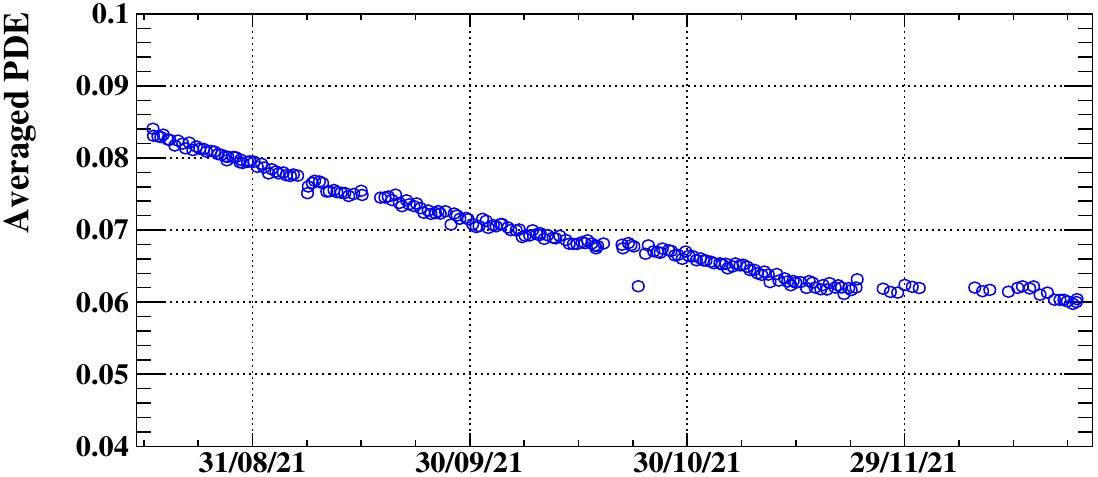
\includegraphics[height=4.4cm]{Figures/MEG/XEC_2021_PDEdecrease.png}\label{fig:MEC:XEC:PDE:drop}}
            \subfloat[PDE recovery thanks to the annealing.]{            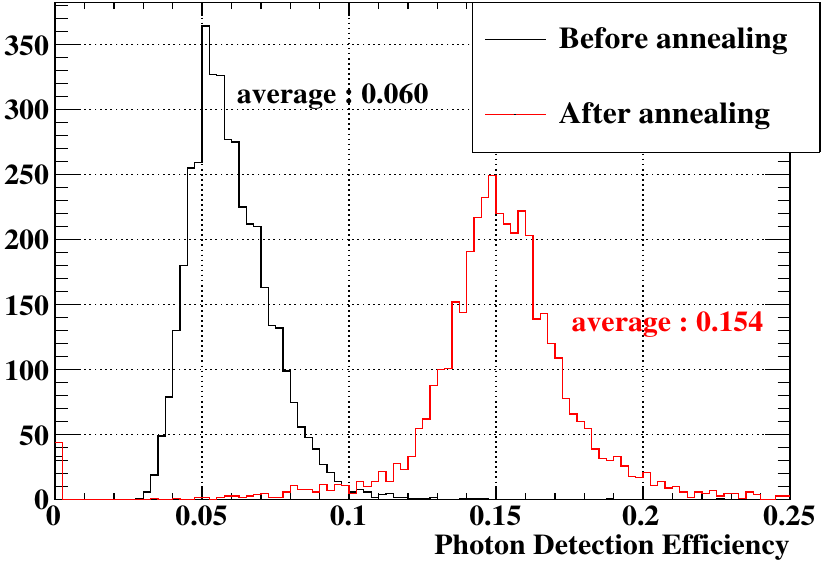
\includegraphics[height=4.3cm]{Figures/MEG/XEC_2022_PDE.png}\label{fig:MEC:XEC:PDE:annealing}}
            \caption{The PDE of the MPPCs was found to be deteriorating due to radiation damage (a). The process of annealing carried out before every physics run, allows the recovery of the PDE (b).}
            \label{fig:MEC:XEC:PDE}
        \end{figure}
        
    \status{review}
    \subsection{Calibration}    
    \label{sec:MEG:XEC:calibrations}
    As anticipated, different calibrations were developed to follow the evolution of the XEC and to tune its functionality. 
    There are three calibrations taken 3/5 times a week plus the Charge EXchange calibration, done once a year.
    
    \paragraph{LEDs} The first of these procedures is done every day, shining the sensor with two different LED lights. 
    This allows us to evaluate the photon detection efficiency (PDE) and Excess Charge Factor (ECF) of the MPPCs.
    The absolute gain of PMTs is also evaluated, with a blue LED, and extrapolating the linear correlation between the mean and variance of the \textit{charge} as a function of the LED intensity. 
    At the beginning of each run, the PMT's gains are set to $\sim\num{0.8e6}$ adjusting the HV. 
    Just like the MPPC PDE, this value will then lower during the run.

    \paragraph{$\upalpha$-particles} PDEs and QEs are evaluated by comparing the number of registered photoelectrons and the expected value, evaluated via MC knowing the positions of the \ce{241Am} source of $\upalpha$-particles.
    The cosmic rays are the background for this calibration and are distinguished via a pulse shape discriminator.
    The uncertainties on the PDEs/QEs is $10\%$.

    \paragraph{\ce{^7Li(p,\g)^8Be}}
    The \SI{17.6}{MeV} line of the \ce{^7Li(p,\g)^8Be} reaction is also used to calibrate the XEC.
    This line is produced impinging a beam of \SI{500}{keV} protons, produced via a Cockcroft-Walton (which will be described in a following section) on a \ce{^7Li} target.

    \paragraph{CEX}
    The last of the calibrations is more complex and requires changing the beam from $\Am$ to $\upmu$. 
    For this reason, it is performed only once a year.
    The process is the Charge EXchange reaction (CEX), $\pi^-p\rightarrow \pi^0n$ and $\pi^0\rightarrow\gamma\gamma$, and produces flat $\gamma$ in $[54.9,82.9]$ MeV.
    Tagging the back-to-back events it is possible to select the low end of the spectrum, which is close to the expected signature of $\Am\ra\Ae\g$ at \SI{52.8}{MeV}. This calibration will be discussed in detail in Ch.~\ref{ch:MEG:CEX}.

    \status{review} 
    \subsection{Reconstruction and performance}
        Let's now discuss how the kinetic variables of the detected $\g$ are extracted and the current understanding of the overall performance of this detector. 
        We will outline the process for the reconstruction without going into details, which can be found in the recent paper \cite{MEG_II:detector}.
        
        \paragraph{Position} The procedure used to find the position $\textbf{x}_\g$ of the hit is based on the assumption the amount of light collected by each sensor is proportional to the solid angle at the interaction point.
        This defines a quantity to minimize, a $\chi^2$ of the registered and expected photons, given the position of each sensor.   
        The position resulting from the fit is then corrected to account for the directionality of the detected photon and the finite size of the EM shower.

        \paragraph{Time} The timing $t_\g$ of the first interaction of the photon is evaluated by minimizing a second $\chi^2$ taking into consideration all the different aspects, like the travel time from the position to the sensors or the offset of each sensor.
        These parameters are evaluated via a dedicated calibration, the Charge EXchange reaction (CEX).
        The results of such a calibration are shown in Fig.~\ref{fig:MEC:XEC:resolution:t}

        \paragraph{Energy} The last ingredient is $E_\g$, which is evaluated as the sum of the number of photoelectrons of each sensor scaled by a factor from $N_\g$ to energy and corrected for a temporal and positional dependence ($T(t), X(u,v,w)$).
        Again, the resolution near the signal energy is evaluated via the CEX. The results are shown in Fig.~\ref{fig:MEC:XEC:resolution:E}.
        The energy scale has been found to be non-uniform. 
        For this reason, a 3D correction $C(x,y,z)$ was developed by joining the information from the CEX runs, the \ce{^7Li(p,\g)^8Be} \SI{17.6}{MeV} line, and the studies of the background.

        \subsubsection{Resolutions} 
        From the analysis of the data collected during the CEX, energy, and timing resolutions can be evaluated near the signal region ($E_{CEX}\sim\SI{55}{MeV}$ \textit{vs} $E_{MEG}\sim\SI{52}{MeV}$).
        The resolutions are extracted by performing a fit, shown in Fig.~\ref{fig:MEC:XEC:resolution} to a double Gaussian for the timing and Eq.~\ref{eq:XEC:E} for the energy.
        For the energy, two regions are necessary because of a low-energy tail originating from the interaction with the detector surface. 
        The resolutions obtained are $\sigma_{E_{\g}}/\mu_{E_{\g}} = 2\%;\ 1.8\%$.
        From design, the relative resolution was expected to be $\sigma_{E_{\g}}/\mu_{E_{\g}} = 2\%;\ 1.7\%$ and the discrepancy is still under study. One possible explanation could be in the behavior of the Xe as a scintillator, given that a similar discrepancy was found also in MEG.
        \begin{equation}
            \label{eq:XEC:E}
            F = 
            \begin{cases} 
                A\exp{-\frac{(x-\mu_{E_\g})^2}{2\sigma_{E_\g}^2}}&\text{if $x>\mu_{E_\g}+\tau$}\\
                A\exp{-\frac{\tau(\tau/2-x+\mu_{E_\g})^2}{\sigma_{E_\g}^2}}&\text{if $x\le\mu_{E_\g}+\tau$}
             \end{cases}
        \end{equation}
    
        \begin{figure}[]   
            \centering
            \subfloat[Time resolution of the XEC, obtained via the time difference of XEC and \textit{pre-shower} fitted with a double Gaussian.]{            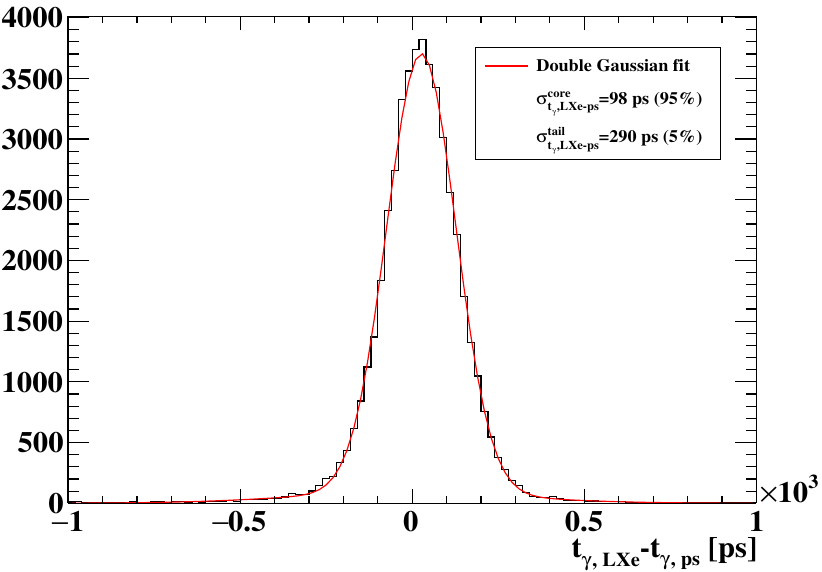
\includegraphics[height=6cm]{Figures/MEG/XEC_t_resolution.png}\label{fig:MEC:XEC:resolution:t}}
            \hfill
            \subfloat[Energy resolution of the XEC.  The function used is Eq.~\ref{eq:XEC:E}.]{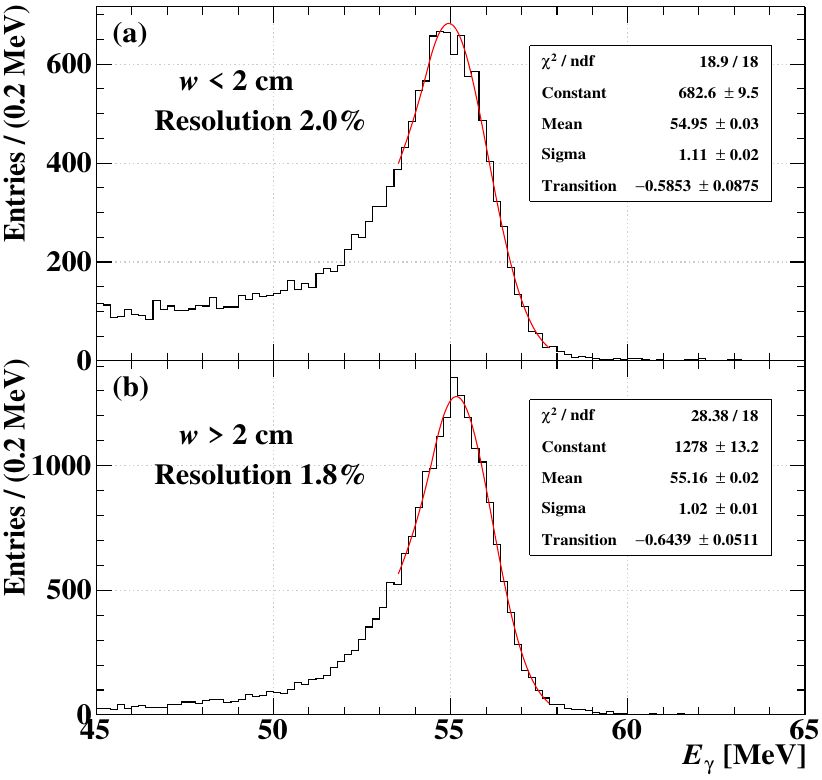
\includegraphics[height=6cm]{Figures/MEG/XEC_E_resolution.png}\label{fig:MEC:XEC:resolution:E}}
            \caption{Timing (a) and energy (b) resolutions of the XEC obtained for \SI{55}{MeV} $\g$s generated via the CEX. The results are for the central region of the detector ($u\in[-10,10]$cm and $v\in[-30,-10]$cm).}
            \label{fig:MEC:XEC:resolution}
        \end{figure}

\status{started}
\section{Spectrometer}
    As already introduced, the spectrometer for the positron's kinematic variables is made of COBRA, CDCH, and pTC.
    We will now review their working principles and designs.

    \status{started}
    \subsection{COBRA}
    \label{MEG:COBRA}
        The COnstant Bending RAdius magnet (COBRA) consists of a main superconducting magnet a two normal conducting compensation coils.
        The main magnet itself is made of five coils with three different radii to generate a carefully studied gradient to achieve two goals:
        \begin{outline}
            \1 Make so that a positron with a given momentum would follow a trajectory of specific radius \textit{independently of the angle} at which the particle has been emitted
            \1 \textit{Quickly} sweep particles emitted at very steep angles, to reduce the pileup
        \end{outline}
        
    \status{started}
    \subsection{Cylindrical Drift CHamber (CDCH)}
        The major difference between MEG's drift chamber and its successor is that the CDCH is a single-volume, replacing the segmented structure.
        This is a $\sim\SI{1.9}{m}$ long cylinder, filled with a helium-isobutane mixture and containing nine concentric layers of 192 gold-plated tungsten wires, which are the heart of this detector.
        While these wires collect the signals from drift electrons, cathode and guard wires ($\sim$10 000 silver-plated aluminum wires) form squared drift cells ranging from \SI{6.6}{mm} to \SI{9.0}{mm}.\\
        The geometry of the CDCH differs slightly from the design.
        For example, 10 layers were planned but 9 were installed due to time limitations. This time was invested in studies to reduce the probability of wire braking.
        This was mainly due to galvanic corrosion of the aluminium core, caused by air humidity penetrating through small cracks in the silver coating.
        The final result after mounting all the wires is shown in Fig.~\ref{fig:MEGII:CDCH}.
        The change in tracking efficiency was studied with simulation yielding a decrease of $< 1\%$.
        Many additional studies can be found in \cite{MEG_II:detector}, like the GARFIELD++ simulations, gas mixtures analysis, and wire tensions.
        To prevent discharges and improve the overall stability, the original He-isobutane gas mixture (90 : 10) was also modified adding a small fraction of oxygen and isopropyl alcohol.\\
        While the 144 HV are supplied with a commercial system, WaveDREAM boards supply the necessary low voltage for the front-end and take care of the digitalization of the waveforms collected at both ends of the wires.

        \begin{figure}
            \centering
            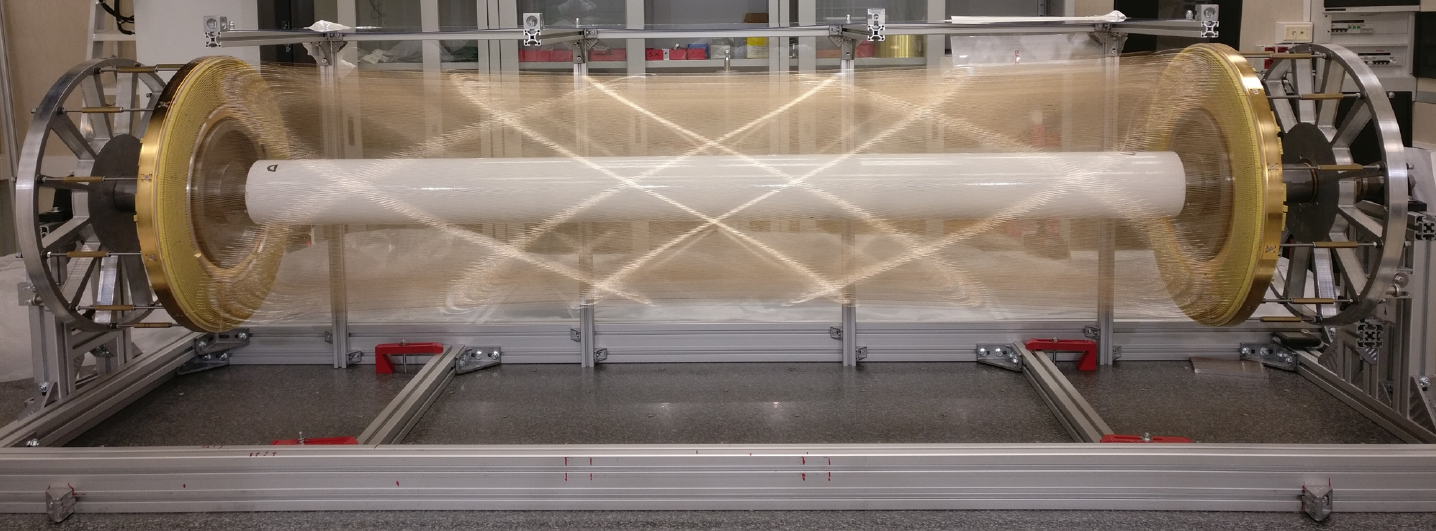
\includegraphics[width = \textwidth]{Figures/MEG/CDCH.png}
            \caption{CDCH with all the wires mounted.}
            \label{fig:MEGII:CDCH}
        \end{figure}

        \paragraph{Hits} The first step in positron tracking is identifying signals (\textit{hits}) induced by drift electrons in the waveforms of the CDCH cells.
        These hits are characterized by multiple pulses from different ionization clusters, stretched due to the slow drift time of electrons.
        Signal-to-noise discrimination and pileup identification are essential. 
        Two waveform processing algorithms have been developed:
        \begin{outline}
            \1 The first algorithm entails two reductions of the noise, fixed voltage thresholds, and integration over 20 ns.
            First, subtraction of a coherent low-frequency noise averaged on adjacent channels (excluding the region with signal pulses).
            This reduces the noise levels from 23 mV to 13 mV.
            Then a high-frequency cut-off at 225 MHz using a discrete Fourier transform technique to eliminate incoherent high-frequency noise.
            \1 The second method utilizes a deep-learning algorithm based on a convolutional neural network (CNN). This CNN model takes waveforms from eight neighboring cells as input and learns the patterns of coherent noise and signals, outputting the probability of the first cluster's arrival time at each sampling point. It is trained using simulated waveform data with randomly added hits and overlaid with real noise data collected without the beam.
        \end{outline}
        
        \noindent
        The second method results in higher hit efficiency but also a higher fake hit rate. 
        To optimize results, the reconstruction process is done once with hits found using the first method and once with hits from both methods combined. 
        The final results are combined after the reconstruction is completed, favoring higher quality tracks if successful with both methods. \\
        The arrival time differences of signals and charges collected at both ends of a wire provide rough (few cm) information about the z-coordinate of the hit along the wire. 
        Stereo wire configuration further improves the z-coordinate resolution.
        This makes the track finding more robust, especially against pileup. \\
        Since multiple clusters often appear on one waveform, identifying the first cluster's time is crucial for correct drift circle reconstruction. 
        The arrival time of the first cluster is determined from the summed waveform of both ends after adjusting their relative timing. 
        The drift time of the first cluster is converted to DOCA using the time-distance relationship (TXY tables).

        \paragraph{Track} After identifying and reconstructing hits, a pattern recognition algorithm (track finder) and a track-fitter algorithm, both based on Kalman filters\footnote{The Kalman filter is a recursive procedure to `bend' the result of a fit. A simple example explanation and an example in 2D are shown in App.~\ref{ch:Kalman}, taken from \cite{mythesis}}, are employed:

        \begin{outline}
            \1 The track finder initiates from hit pairs in outer layers with lower occupancy and generates track seeds by combining compatible pairs from different layers. 
            Each seed is propagated through adjacent layers, checking consistency with hits and updating track parameters. 
            Candidates with at least seven hits are formed.
            \1 The track fitter utilizes an extension of the Kalman filter called the deterministic annealing filter (DAF) and resolves left/right ambiguities. 
            It fits individual track candidates from the track finder, combining segments to form multi-turn tracks within CDCH. 
            Tracks are propagated to the pTC and backward to the target, with re-fitting based on updated DOCA using the best-estimated T0.
        \end{outline}

        \noindent
        During tracking, DOCA of each hit is iteratively refined. Initial DOCA values are estimated from Garfield++ simulations, but they can be biased due to low cluster density. 
        An alternative DOCA estimate is obtained through neural network approaches, providing a more accurate estimation and improving positron kinematics by about 10\%. 
        This CNN-based method is used for final DOCA estimation during the re-fit process.


        \paragraph{Perfomrance and efficiency}

        \begin{figure}
            \centering
            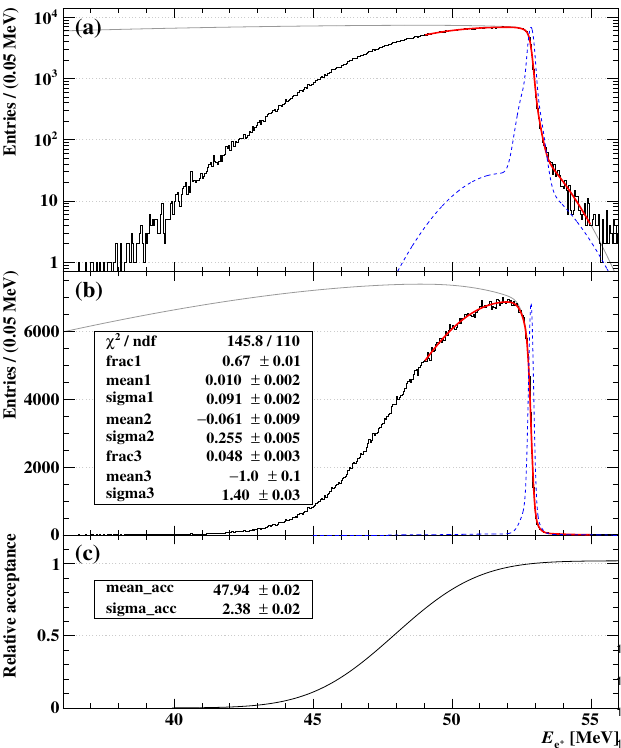
\includegraphics[width = 0.48\textwidth]{Figures/MEG/CDCH_michelfit.png}
            \caption{Michel positron spectrum in logarithmic (a) and linear (b) scales. Black - data; Blue - 3 Gaussians to describe the resolution; Red- fit. The acceptance curve is shown in (c).}
            \label{fig:MEGII:CDCH:michel}
        \end{figure}

        \paragraph{CDCH2} The studies prompted by the wire breakage evolved in an R\&D for the updated version of the CDCH. The main change was the choice of pure aluminum \SI{50}{\micro m} wires,  almost insensitive to corrosion.
        One of the main challenges spawned by this choice was to develop a solid way of fixing the wires to the PCBs: the solution found was a combination of soldering and gluing.
        The CDCH2 will be completed by the end of 2023 and delivered to PSI in spring 2024.
        The choice of mounting the new system will then depend on the current status and stability of the CDCH.

    \status{started}
    \subsection{pixelated Timing Counter (pTC)}
        The time coincidence between $\Ae$ and $\g$ is crucial at high $R_\upmu$. 
        The pixellated Timing Counter plays two roles: first, it is part of the trigger algorithms; second it assigns the time of the positron track, which is then propagated backward to the target plane $t_{\Ae}$. 
        This detector is made of two symmetric half-cylinders of scintillators between the CDCH and COBRA, as shown in Fig.~\ref{fig:MEGII:pTC}.
        To cover the $\Ae$ acceptance corresponding to a $\g$ entering the XEC, the pTC covers : $\SI{23}{cm}<\abs{z}<\SI{117}{cm}$ and $\SI{-166}{\deg}<\phi<\SI{5}{\deg}$. 
        Each sector is made of 256 Bicron \bc{422} plastic scintillators read on opposite sides by arrays of 6 AdvanSiD $3\times3$ mm SiPM, as shown in Fig.~\ref{fig:MEGII:pTC:tile}.
        The tiles are wrapped in \SI{35}{\micro m} polymeric reflector and \SI{30}{\micro m} \tedlar.\\
        The size and location of the tiles were optimized with ad hoc simulations: two different sizes ($120\times40/50\times5$ mm$^3$)  are placed in a $16\times16$ matrix in the $z\phi$ plane and tilted by \SI{45}{\deg} to be orthogonal to the positron trajectories.
        This configuration was chosen to maximize the multiplicity for signal-like positrons limiting the material budget.
        The mean multiplicity from MC is $\langle N_{hit} \rangle\sim 9$ and the obtained resolution $\sigma_{t_{\Ae}, pTC} \sim \SI{40}{\pico s}$.
        To intercalibrate the timing offsets of the system, most tiles are lit with a synchronous light pulse via optical fibers.
        
        \paragraph{Performance} The single-counter time resolutions were measured to be $\sigma_{t_{\Ae}, pTC}(N_{\text{hit}} = 1) \sim 80-120$ ps for counters with heights of 40 mm and 50 mm. These resolutions correlate with light yield, influenced by scintillator aging, SiPM detachment, and radiation damage.
        Multi-hit time resolution is assessed via the "even-odd" method, improving average resolution to $\sigma_{t_{\Ae}, pTC} = 43$ ps by combining results from different hit groups. 
        Efficiency of $pTC$ was studied with MC simulation, yielding a total detection efficiency of $\epsilon_{e^+, pTC} = (91 \pm 2)\%$, considering factors like geometric acceptance and scattering effects on endcaps.

        \begin{figure}
            \centering
            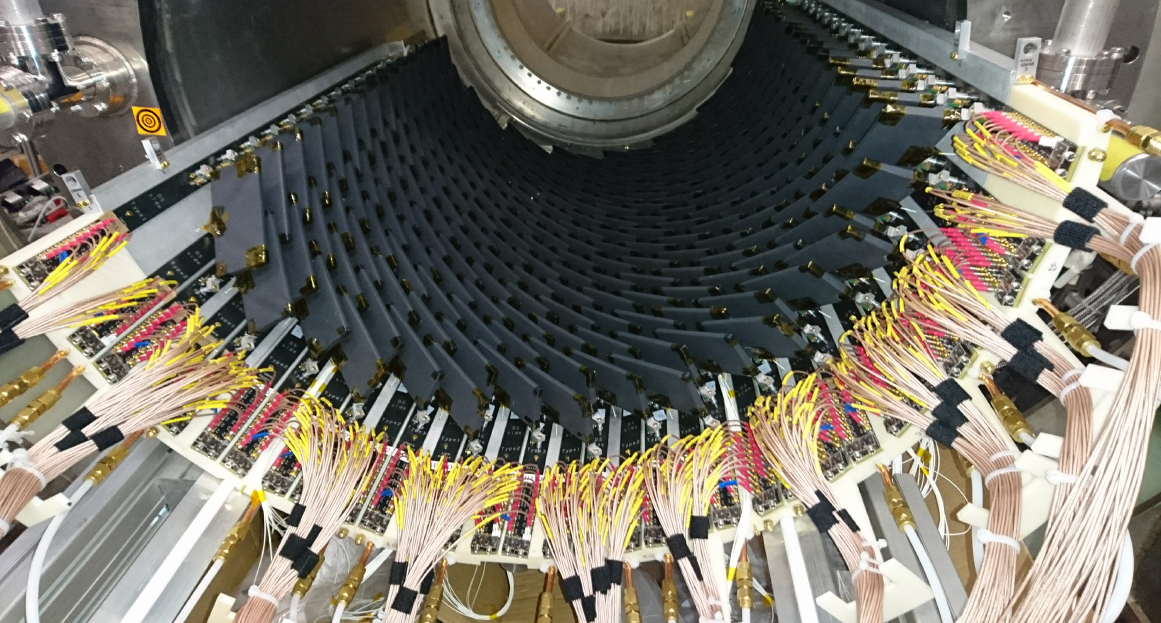
\includegraphics[width = 0.8\textwidth]{Figures/MEG/pTC.png}
            \caption{}
            \label{fig:MEGII:pTC}
        \end{figure}

        \begin{figure}
            \centering
            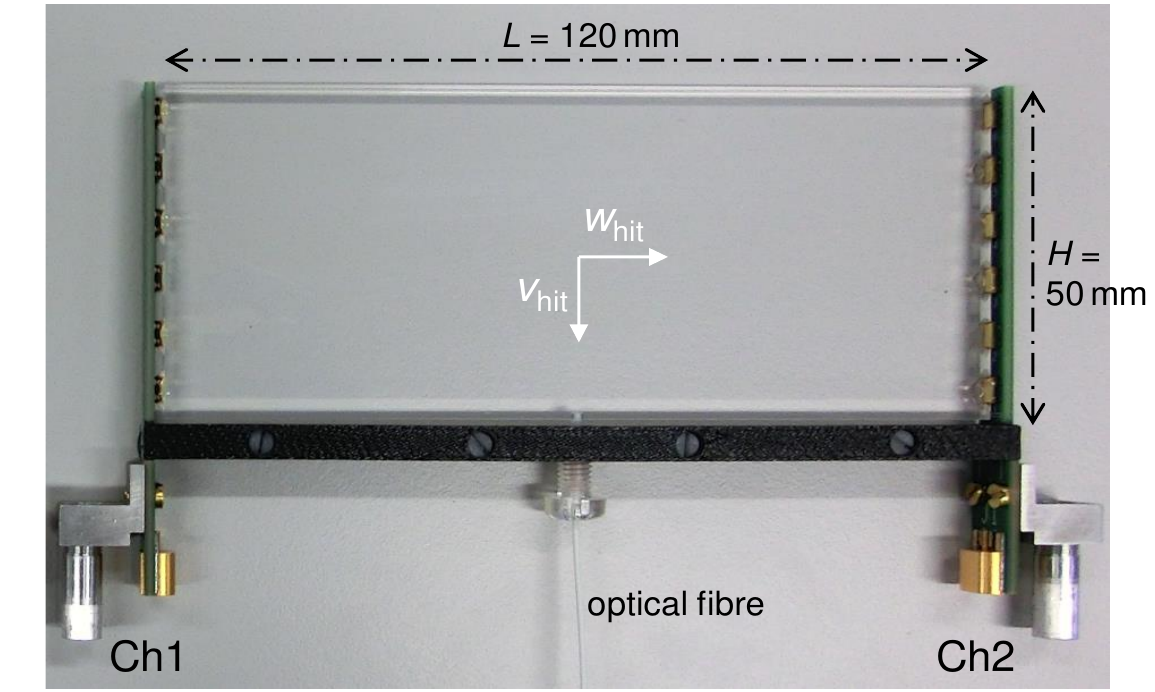
\includegraphics[width = 0.8\textwidth]{Figures/MEG/pTC_tile.png}
            \caption{A pTC tile: $120\times40/50\times5$ mm$^3$ of \bc{422} read by arrays of 6 AdvanSiD $3\times3$ mm SiPM.}
            \label{fig:MEGII:pTC:tile}
        \end{figure}

        \begin{figure}
            \centering
            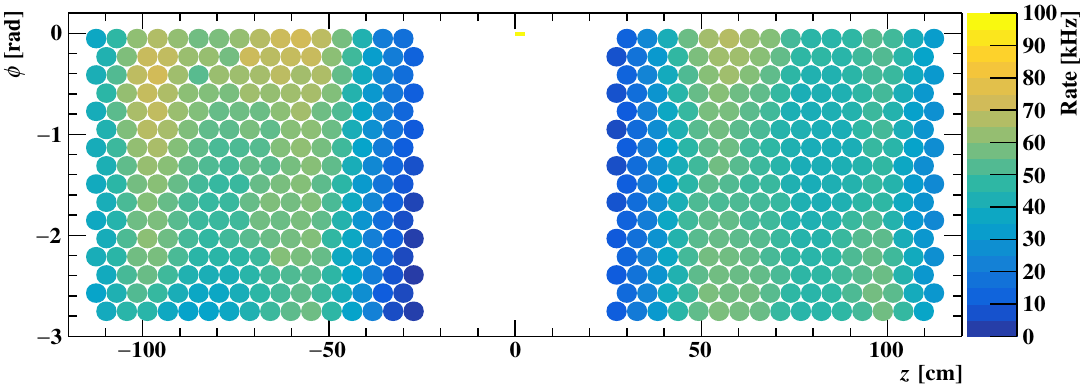
\includegraphics[width = \textwidth]{Figures/MEG/pTC_rate.png}
            \caption{Hit rates map of the pTC at $R_\upmu = \SI{5e7}{\upmu \per s}$ during the 2022 run. Each circle indicates a counter.}
            \label{fig:MEGII:pTC:rate}
        \end{figure}
        
\section{Trigger and DAQ}

\status{review}
\section{Beam and target}
    The beamlines at PSI were described in \ref{intro:beamlines}. 
    The beamline delivering $\mu^+$ to MEG II, in particular, is the $\pi E5$ line, shown in  Fig. \ref{fig:pie5}.
    The design, tuning, and deep understanding of this line play a key role in the success of the MEG experiment. 
    Here we will describe the beamline, outline the key elements, and the related simulations. 
    We will then describe the MEG II target, with some detail on the way to take into account its deformations during the analysis.

    \status{review}
    \subsection{$\pi E5$}
        This beam-line has actually two possible configurations: this will allow the area to be shared between MEG II and Mu3e. 
        As already illustrated, the surface muons delivered by this beam-line are produced for the decay of the pions generated as secondary beams from the HIPA proton beam.
        On top of muons, pions, and positrons also are transported by the beamline.
        We will briefly describe the elements of $\pi E5$ (COBRA has been already described). 

        \begin{outline}
            \1 AHSW41 dipole: Captures the pions and muons in the backward direction and defines the momentum acceptance of the beamline.
            \1 Straight section: Quadrupoles (QSF4*), sextupoles (HSC4*) and three slits (FS41–42–43) shape the beam. FS41 In particular is used to reduce the beam intensity and momentum spread.
            \1 AST41 dipole: This element is used to define in which channel the beam is sent. "Z" channel for MEG II and "U" channel for (the upcoming) Mu3e.
            \1 Separator: The beam arrives in a Wien filter via Triplet I and a quadrupole triplet. Te aim is to separate the muons from pions and positrons.
            \1 Triplet II at a collimator: This pair focuses the beam and cuts the tails.
            \1 BTS: This Beam Transport Solenoid contains a \SI{300}{\micro m} thick \mylar moderator.
            \1 A \SI{190}{\micro m} \mylar window separates the beampipe from the He atmosphere in COBRA.
            \1 COBRA: The design choice for this element was previously illustrated (\ref{MEG:COBRA}). 
            The behavior of the beam inside this element is quite tricky to simulate consistently.
        \end{outline}

        \noindent
        Although not one of my tasks, I helped during some of the beam tuning done during these last years.
        Aside from the beginning of the run, these elements are tuned also when there is a major change in the main proton beam, often related to the overall current of incoming particles.
        Another tune is done at the end of the year to change the beam from $\Am$ to $\uppi$, necessary for the CEX.
        
        \paragraph{Beam profile}
        In Fig.~\ref{fig:meg:beamprofile} is shown a typical beam profile at COBRA center: The beam is in $x_b = \SI{0.0(5)}{mm}$, $y_b = \SI{-0.8(5)}{mm}$ with standard deviations $\sigma_x = \SI{11.35(50)}{mm}$ and $\sigma_y = \SI{11.36(50)}{mm}$. 
        This beam was measured with slits such as the stopped muon rate was $R_\upmu = \SI{5.3e7}{\upmu \per s}$ at the primary proton beam current $I_p = \SI{2.2}{mA}$. 
        Similar profiles were achieved in the range $R_\upmu = (2 \divisionsymbol 5) \times \SI{e7}{\upmu \per s}$.
        The measurements on the stopped muon rate are evaluated using the stopping efficiency extracted by simulations (89\%) and are affected by a 5\% uncertainty due to the variations of the proton beam position on Target E.

        \begin{figure}
            \centering
            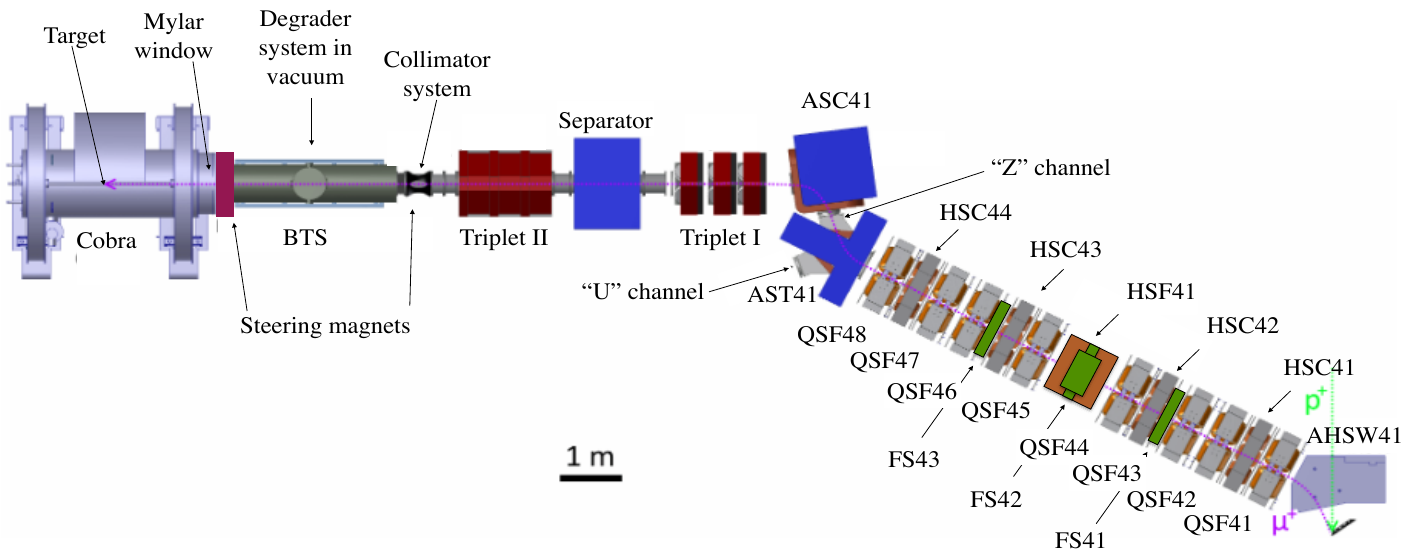
\includegraphics[width = \textwidth]{Figures/MEG/piE5_beamline.png}
            \caption{Detail sketch of the $\pi E5$ beamline at PSI.}
            \label{fig:pie5}
        \end{figure}
        
        \begin{figure}
            \centering
            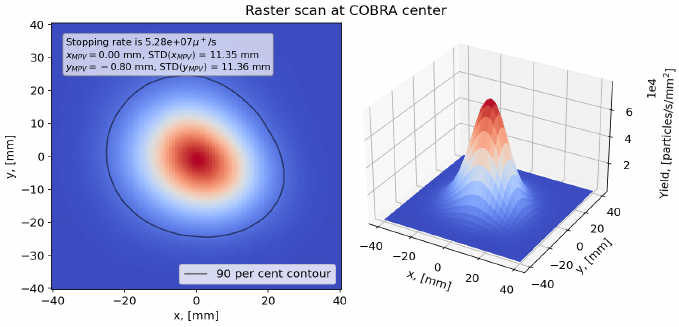
\includegraphics[width = 0.8\textwidth]{Figures/MEG/meg_beamprofile.png}
            \caption{Beam profile at COBRA center for a stopped muon rate of $R_\upmu = \SI{5.3e7}{\upmu \per \second}$ at $I_p = \SI{2.2}{mA}$.}
            \label{fig:meg:beamprofile}
        \end{figure}

    \status{review}
    \subsection{Simulations}
        As introduced in the previous section, the understanding of the beam behavior is a key aspect of the experiment.
        The beamline itself was developed using TRANSPORT, a beam optics simulation program.
        The model was later implemented in \gfb\footnote{\gfb is a simulation program for particle physics based on \gf and can be found \href{https://www.muonsinc.com/Website1/G4beamline}{\underline{here}}.}.
        The reason to have a physics-based simulation on top of the optics simulation is quite obvious: optics programs cannot simulate interaction with materials and all the physical processes taking place in a beamline.

        
        \paragraph{\gfb} Being based on \gf, this program is a flexible and extensible framework for implementing complex simulations of particle interactions, including electromagnetic and hadronic processes, decay processes, and tracking in magnetic fields.
        Just like \gf, the simulation is run particle by particle and \textit{step}-based.
        This means that at every interaction physical models are used to update the particle state and generate necessary secondary particles.
        The major extensions in \gfb are predefined beamline elements, beam generators, and some optic tools to study the performance of the beamline.
        An example of particle tracking in this program is shown in Fig.~\ref{fig:piE5_gfb}.
        In the last years this simulation has been updated and developed by Giovanni Dal Maso to extract the best possible understanding of the stopped muon rate $R_\upmu$. 

        \begin{figure}
            \centering
            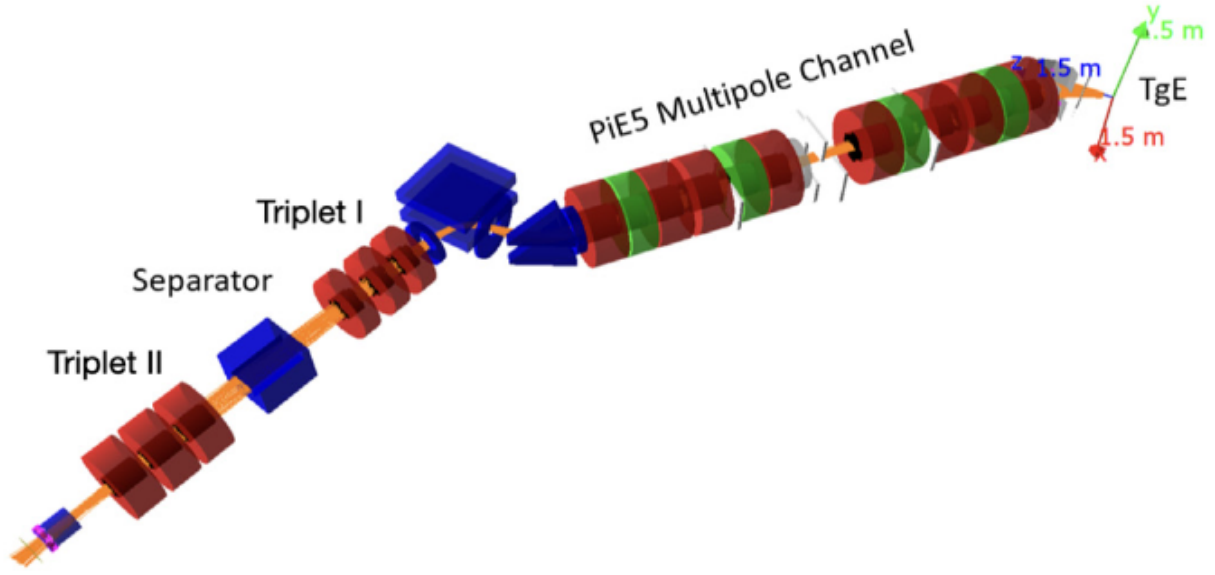
\includegraphics[width = \textwidth]{Figures/MEG/piE5_gfb.png}
            \caption{\gfb simulation of few tracks (orange lines) in the $\pi E5$ beamline. It's possible to recognize the elements discussed previously and showed in Fig~\ref{fig:pie5}.}
            \label{fig:piE5_gfb}
        \end{figure}
        
        \paragraph{\madx} During 2022/2023 Luca Biasia, a Master student in Pisa, developed a \madx\footnote{\madx is a general-purpose tool for charged-particle optics design and can be found \href{http://madx.web.cern.ch/madx/}{\underline{here}}.} simulation to describe the $\pi E5$ line and cross-validate the results obtained using \gfb and to start the transition from TRANSPORT to \madx.        
        My contribution to this simulation was only partial: I provided Luca with some working \madx examples, developed while attending the JUAS, and some initial help for him to start playing with this simulation framework. 
        After this initial `starting kit', Giovanni Dal Maso was the one overseeing the development while I only followed the updates and gave feedback or suggestions. \\
        After a comparison with data and \gfb some discrepancies arose and, after many iterations, they were associated with the description of the fringing fields of the components in \madx. 
        The solution adopted was to slice the field maps in thin layers and define many thin `\madx elements'. 
        A comparison of the results from QSK41 to COBRA center is shown in Fig.~\ref{fig:madx_vs_g4b}.
        During the beam tuning in June 2023, this simulation was crosschecked: after measuring the beam spot at COBRA center the currents of the magnets were chosen with \madx to obtain a different beam shape. 
        The measurement was consistent with the resulting simulation.
        This was a great achievement and, moving forward, this tool is going to play a key role during the beam tuning.

        \begin{figure}
            \centering
            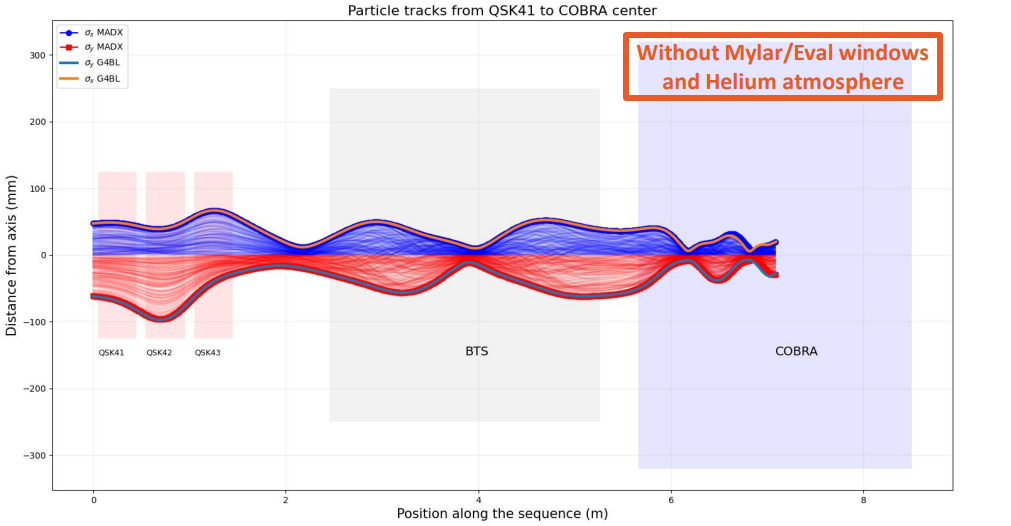
\includegraphics[width = \textwidth]{Figures/MEG/madx_vs_g4b.png}
            \caption{Comperison of the results from the \gfb and \madx simulations for $\pi E5$. While the agreement is very good for most of the beamline, there is some difference inside COBRA. This is due to the difficulty in describing the highly `non-standard' magnet. Given \madx has no particle interaction, the comparison is fair only when removing all materials from the beamline in the \gfb simulation.}
            \label{fig:madx_vs_g4b}
        \end{figure}

    \status{review}
    \subsection{MEG II target}
        The aim of the target is to stop $\Am$ at COBRA center while minimizing the interaction of the secondary particles produced.
        The knowledge of the position of the target and planarity are key components in evaluating the systematic errors on the reconstructed vertex position. 
        After in-depth studies, the BC400 scintillating plastic was selected as the material for the target.
        The shape is a ellipse of $\SI{270}{mm}\times\SI{66}{mm}$ and \SI{170}{\micro m} thick, with a maximum variation of \SI{20}{\micro m}. 
        The target is inclined such as the normal of its surface creates a \SI{75.0(1)}{\degree} angle with the beam. 
        
        \paragraph{Deformation and pictures} In order to identify the $\Am\ra\Ae\g$ process, it is necessary to measure the angles $(\phi_e,\theta_e)$ at the target, back-propagating the reconstructed tracks.
        The resolution on these variables is $\sim\SI{7}{m rad}$, but a simple displacement of \SI{500}{\micro m} of the target propagates as systematics of $\ge \SI{4}{mrad}$ on $\phi_e$.
        For this reason, the collaboration developed three different ways of keeping these systematics under control:
        \begin{outline}
            \1 A yearly optical survey to measure the position inside COBRA.
            \1 Fiducial holes in the target: This allows to study the position of the target reconstructing the position of the vertices for many events, but it requires months of data. 
            \1 Photogrammetric survey of a dot pattern on the target itself.
        \end{outline}
        \noindent
        While the first two were used already in MEG, the third was developed for the upgraded MEG II.
        A picture of the target is in Fig.~\ref{fig:meg:target}, where the dot pattern is clearly visible.
        Two different CMOS cameras are used to take pictures of the target and two different methods are then employed to study the sequence of pictures.
        The position of the center of the target is described in the MEG II coordinate system, while the deformation is accounted for differently by the two methods:
        \begin{outline}
            \1 In the first method, $\chi^2$ is evaluated between the measured and expected dot positions. The expected positions depend on the position of the target, the deformation (parametrized with Zernike\footnote{Zernike polynomials are a set of orthogonal functions commonly used in optics and image analysis (see \href{https://en.wikipedia.org/wiki/Zernike_polynomials}{\underline{Wikipedia}}).} polynomials), and the optical parameters of the system. 
            \1 The second method minimizes the $\chi^2$ for the observed and measured 2D positions of the dots on the camera plane. Clearly, the optical projection on this plane is the cardinal element.
        \end{outline}
        These two methods have been proven to be compatible within \SI{100}{\micro m}.
        
        \begin{figure}
            \centering
            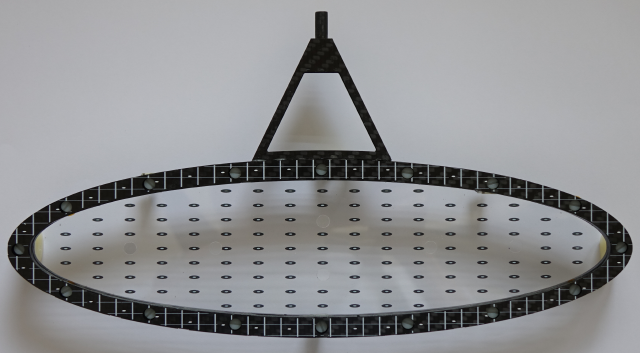
\includegraphics[width = 0.8\textwidth]{Figures/MEG/meg_target.png}
            \caption{Picture of the BC400 target. Clearly visible is the dot pattern on both the target and carbon fiber frame. Six holes, admittedly less visible, are located on the axes of the ellipse.}
            \label{fig:meg:target}
        \end{figure}

        \begin{figure}   
            \centering
            \subfloat[Example of a photon detected by the XEC.]{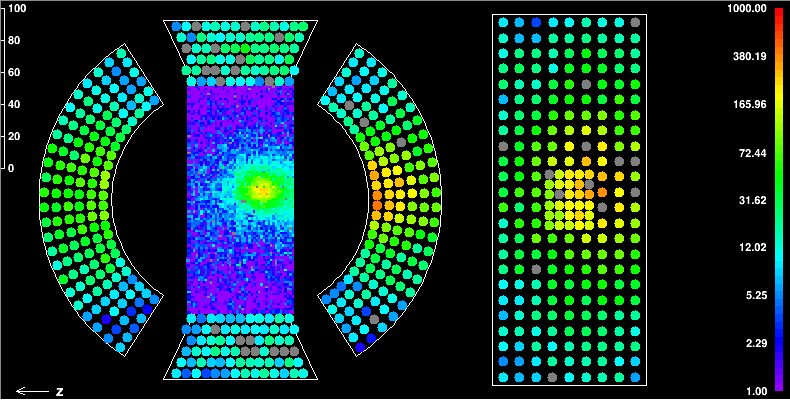
\includegraphics[width=\textwidth]{Figures/MEG/XEC_example.png}\label{}}\\
            \subfloat[Example of a $\Ae$ detected by the pTC.]{            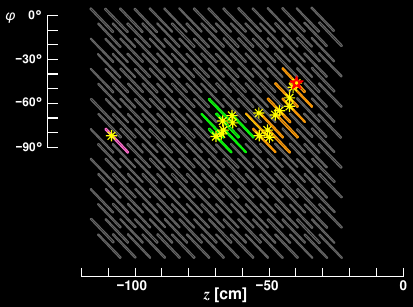
\includegraphics[height=6.3cm]{Figures/MEG/pTC_example.png}\label{}}
            \hfill
            \subfloat[Example of a $\Ae$ detected by the CDCH. AAA WRONG]{            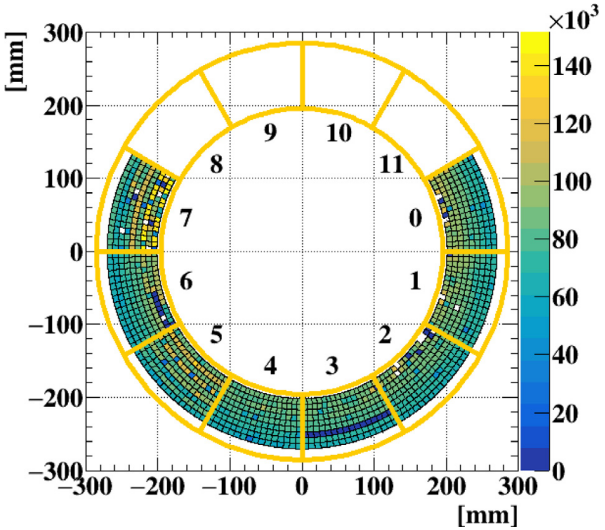
\includegraphics[height=6.6cm]{Figures/MEG/CDCH_example.png}\label{}}
            \caption{}
        \end{figure}
        
\status{review}
\section{Cockcroft–Walton}
    \label{sec:cw:calib}
    In addition to the muon beamline, MEG II has a Cockcroft–Walton proton accelerator. 
    After the description of the machine, we will highlight the use of this accelerator by the collaboration (calibrations of the XEC and exotic searches) and the recent maintenance.
    One of my main tasks during this Ph.D. has been the usage of this machine, so I was quite fortunate to be able to shadow the expert during the maintenance.

    \status{review}
    \subsection{Description of the machine}
        \label{sec:cw:machine}
        The accelerator is a single-stage in-line singletron produced by HVEE. 
        This machine is a compact Cockcroft–Walton with a terminal voltage of $0.1\divisionsymbol1.0$ MV and a proton current up to \SI{100}{mA}.
        
        \paragraph{Source} The RF ion source is a bottle of gas that is excited by an RF oscillator. 
        The electrons in the gas are excited and, because of the collisions with the neutral gas particles, cause ionization.
        The plasma produced is confined with an axial magnetic field and serves as the source of positive ions, which are extracted by applying a DC electric field.
        A schematic of the working principle of the RF ion source is shown in Fig.~\ref{fig:CW:sketch:ionsource}

       \begin{figure}
            \centering
            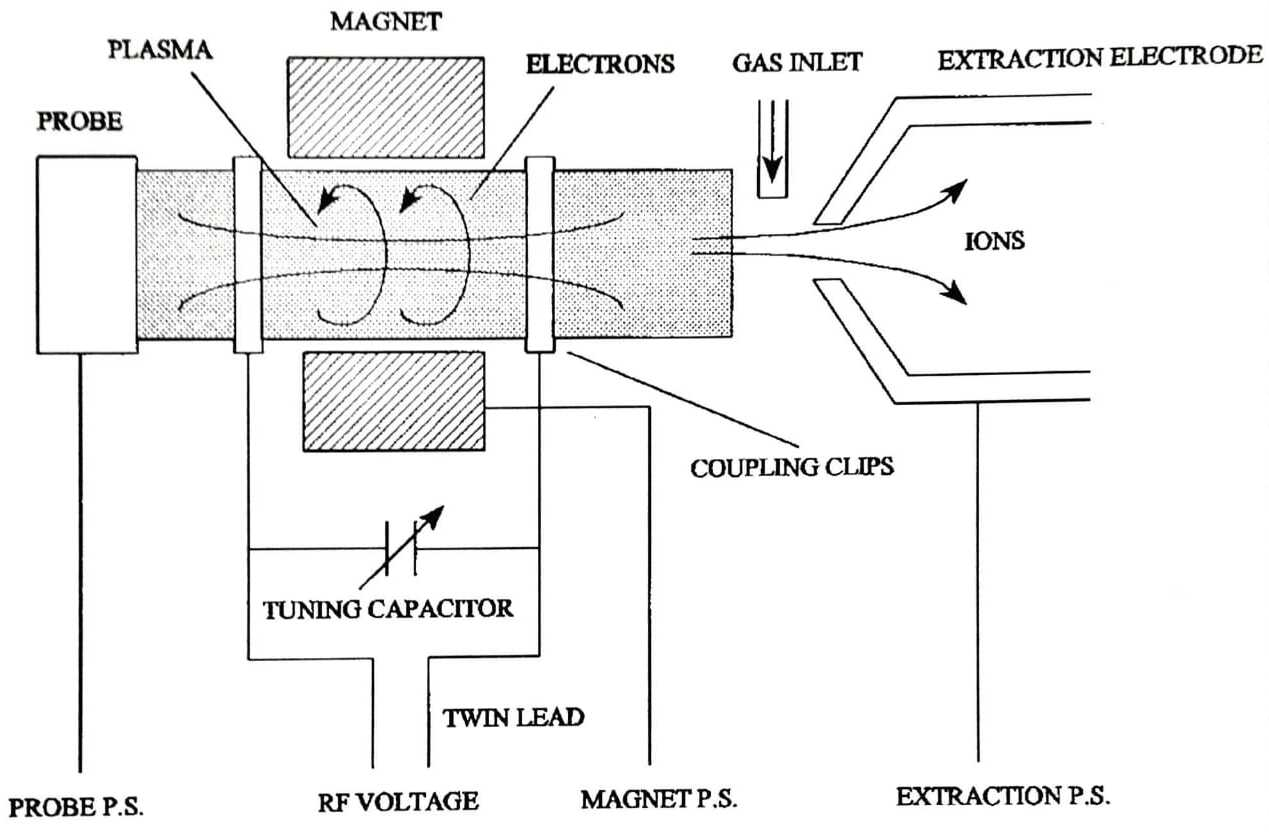
\includegraphics[width=0.8\textwidth]{Figures/MEG/CW/cw_ionsource.jpeg}
            \caption{Sketch of the ion source of the CW.}
            \label{fig:CW:sketch:ionsource}
        \end{figure}
        
        \paragraph{CW-Circuit}
        The high-voltage multiplier and rectifier stack, together with the RF driver and HV control and stabilizing system, is one of the core sections of the machine.
        It is located in the main pressure tank, while the RF resonance coils are in a separate \ce{SF6} filled tank and the RF driver in a separate cabinet.
        This gas is often used as a gaseous dielectric medium because of its high dielectric strength, the result of the gas's high electronegativity
        \footnote{Electronegativity is a measure of the attraction of an atom for bonding electrons in molecules compared to that of other atoms: large values indicate a stronger attraction and it increases from left to right across the periodic table.} and density.
        In the case of an arc, \ce{SF6} can break down in different ways but most of the decomposition products tend to quickly re-form \ce{SF6}, a process termed \textit{self-healing}. 
        Arcing or corona can also produce disulfur decafluoride (\ce{S2F10}), a highly toxic gas, which is the reason extra care is needed when opening such a system.
        This stack is a parallel-fed CW power supply that consists of a series of high voltage rectifiers and capacitive coupling \textit{corona} rings.
        The power is fed via an RF driver capacitive coupled.
        A sketch of the inner structure of a rectifier assembly (\textit{ass'y}) is shown in Fig.~\ref{fig:CW:sketch:rectifier} while in Fig.~\ref{fig:CW:removal} is clearly visible the way the ass'ys are mounted.

        \begin{figure}[ht]   
            \centering
            \subfloat[Schematic of power supply.]{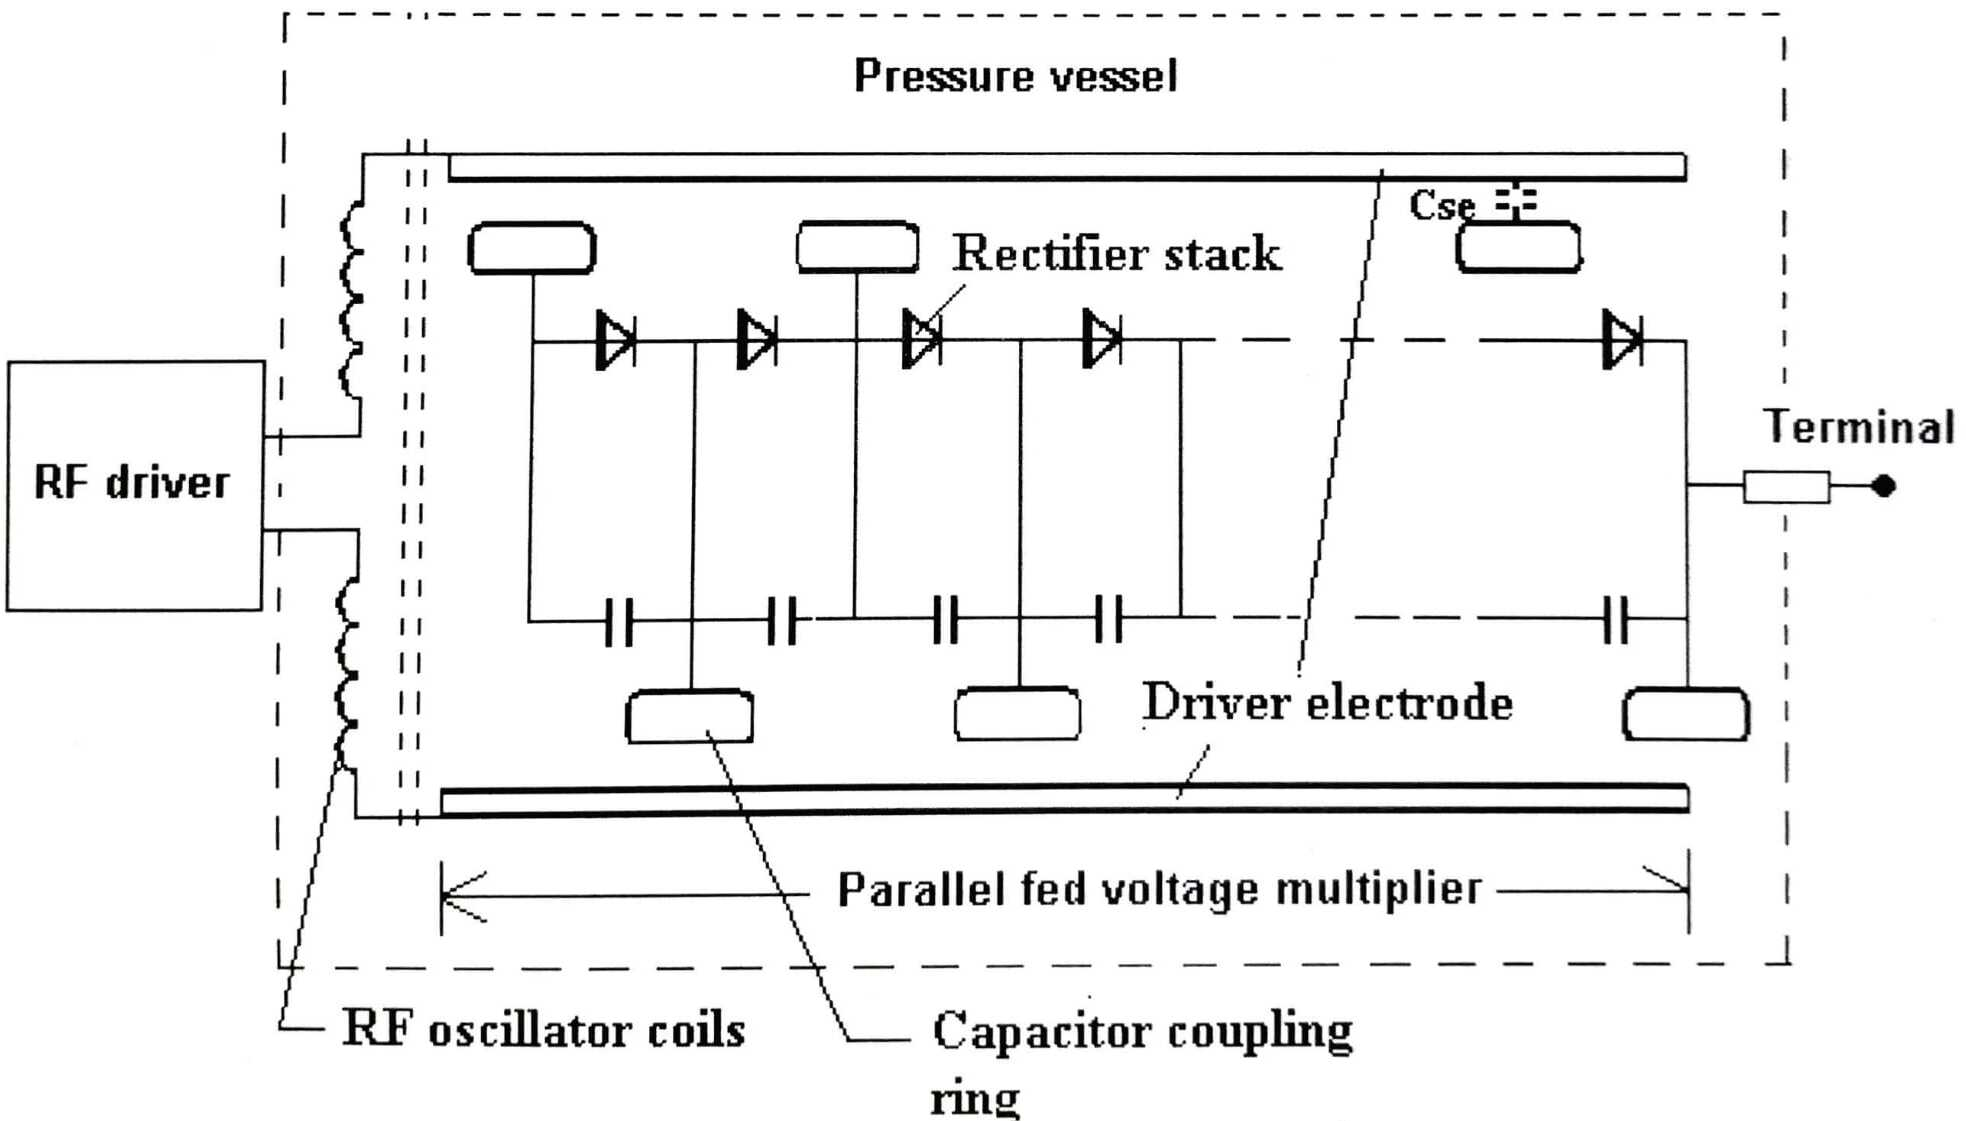
\includegraphics[width=0.8\textwidth]{Figures/MEG/CW/cw_circuit_stack.jpeg}\label{fig:CW:circuit:stack}}\\
            \subfloat[Sketch of the inner structure of a \textit{stack ass'y}: 15 rectifiers and 2 resistors.]{            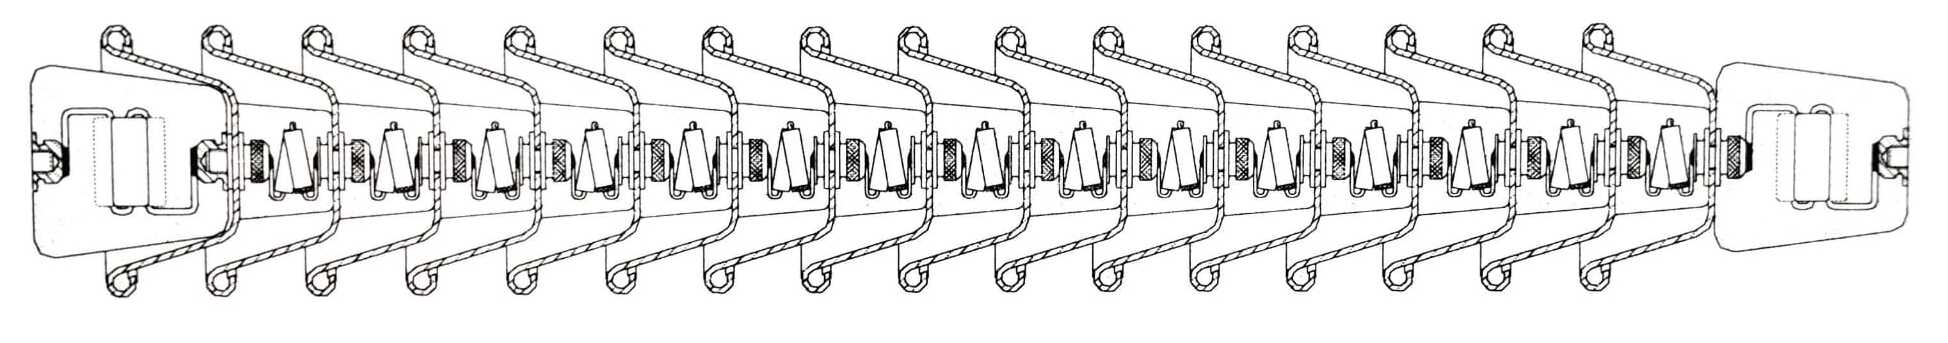
\includegraphics[width=0.8\textwidth]{Figures/MEG/CW/cw_rectifier.jpeg}\label{fig:CW:sketch:rectifier}}
            \caption{The first schematic (a) shows the CW circuit and the capacitive coupling to the RF driver while the second (b) shows the internal structure of a rectifier stack (\textit{stack ass'y}).}
        \end{figure}

        \paragraph{Driver}
        The driver, as the name suggests, is the circuit that feeds the voltage/power to the whole system.
        In between the driver and the CW stack of rectifiers' ass'ys a resonant circuit is used to amplify the output of the driver.
        The power is fed to this resonant circuit in phase with the oscillating current.
        Keeping the frequency at resonance, the driver controls the terminal voltage adjusting the pulse width.
        A block diagram of the driver is shown in Fig.~\ref{fig:CW:circuit:driver}

        \begin{figure}
            \centering
            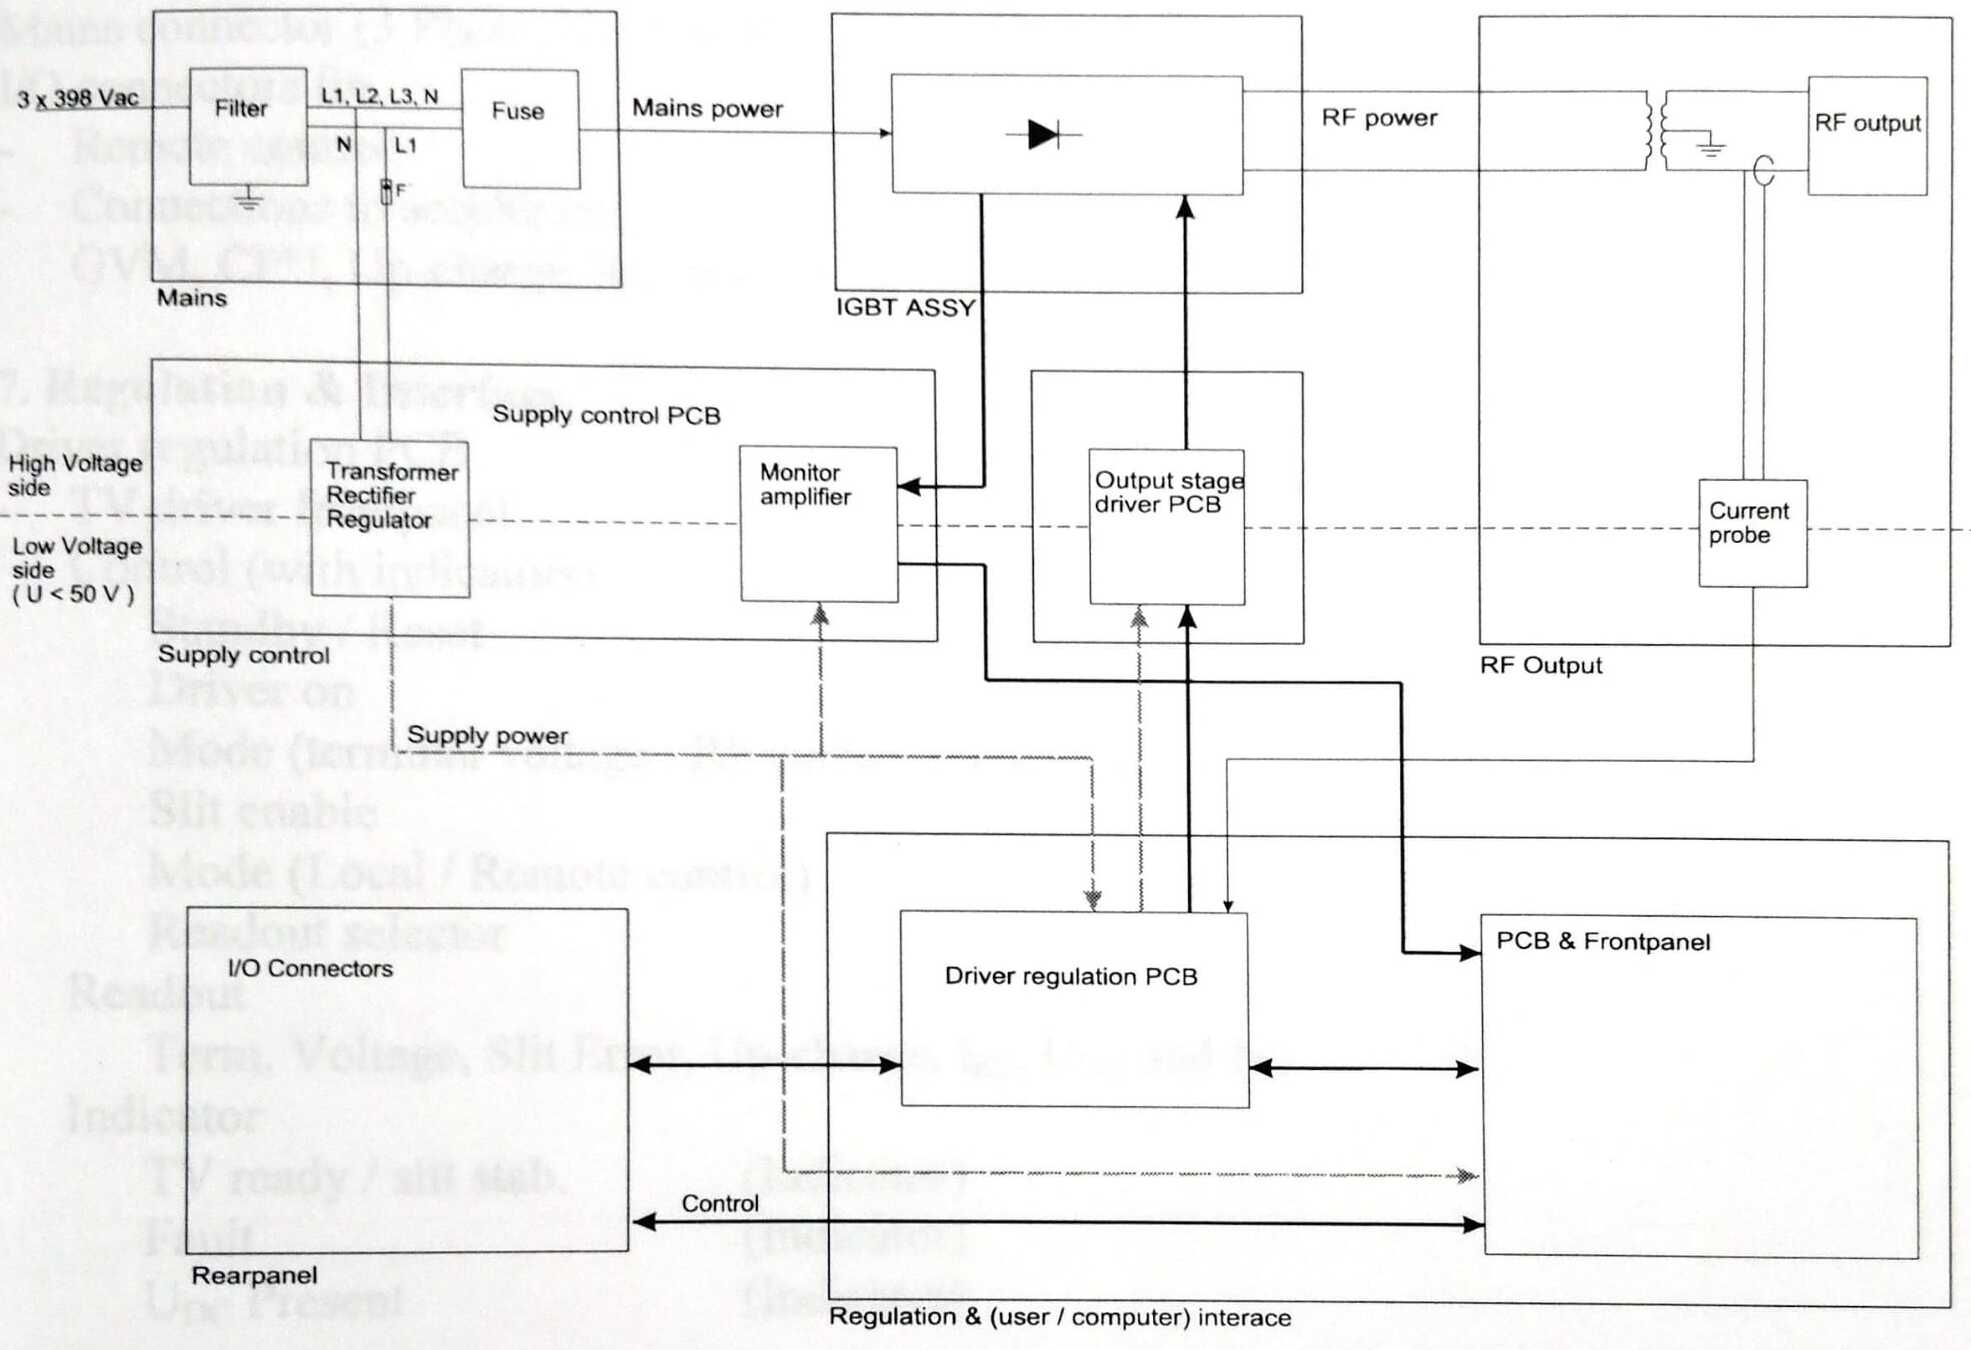
\includegraphics[width=0.8\textwidth]{Figures/MEG/CW/cw_circuit_driver.jpeg}
            \caption{Block diagram of the driver}
            \label{fig:CW:circuit:driver}
        \end{figure}

        \paragraph{Start-frequency}
        The system can operate only at resonance and this frequency $f_{res}$ is defined by the coil and dynodes.
        During star-up, the system starts at $f_{start}$ higher than the resonance and then lowers it until the resonance is found.
        A parasitic frequency $f_{par}$, with $f_{par}>f_{res}$, is also present. 
        At this frequency, the driver oscillates at a higher frequency, and no power is transferred to the terminal.
        To avoid the higher frequency, a tuning is needed so that $f_{par}>f_{start}>f_{res}$.

        
        \paragraph{Q-factor} In the RF resonance circuit high amounts of 'blind power' can be present (up to \SI{1}{MW}).
        The quality factor (Q-factor) of the RF resonance circuit is the ratio of blind to dissipated power.
        E.g. for a blind power of \SI{1}{MW} and a Q-factor of 1000 the transformer coil dissipates \SI{1}{kW} of heat.
        If this factor is not high enough the dissipated power is too high and will prevent the driver from operating correctly.
        The Q-factor is measured using a function generator and looking at the relative phase and amplitude of voltage in two points of the accelerator's RF resonance circuit.
        A sketch of the measurement is shown in Fig.~\ref{fig:CW:sketch:Q-factor}.
        The system is at resonance when there is no relative phase between $V_1$ and $V_2$, and the value of $V_1/V_2$ is used to evaluate the Q-factor: 
        \begin{equation}
            Q = Z_{coil}/R_{loss} = 2\pi f_{req} I_{coil} (V_1/V_2-1)/R_l \approx 43.9\times f_{res}[kHz]\times(V_1/V_2-1)
            \label{eq:cw:qfactor}
        \end{equation}


        \begin{figure}[ht]   
            \centering
            \subfloat[Sketch of the circuit to measure the Q-factor.]{            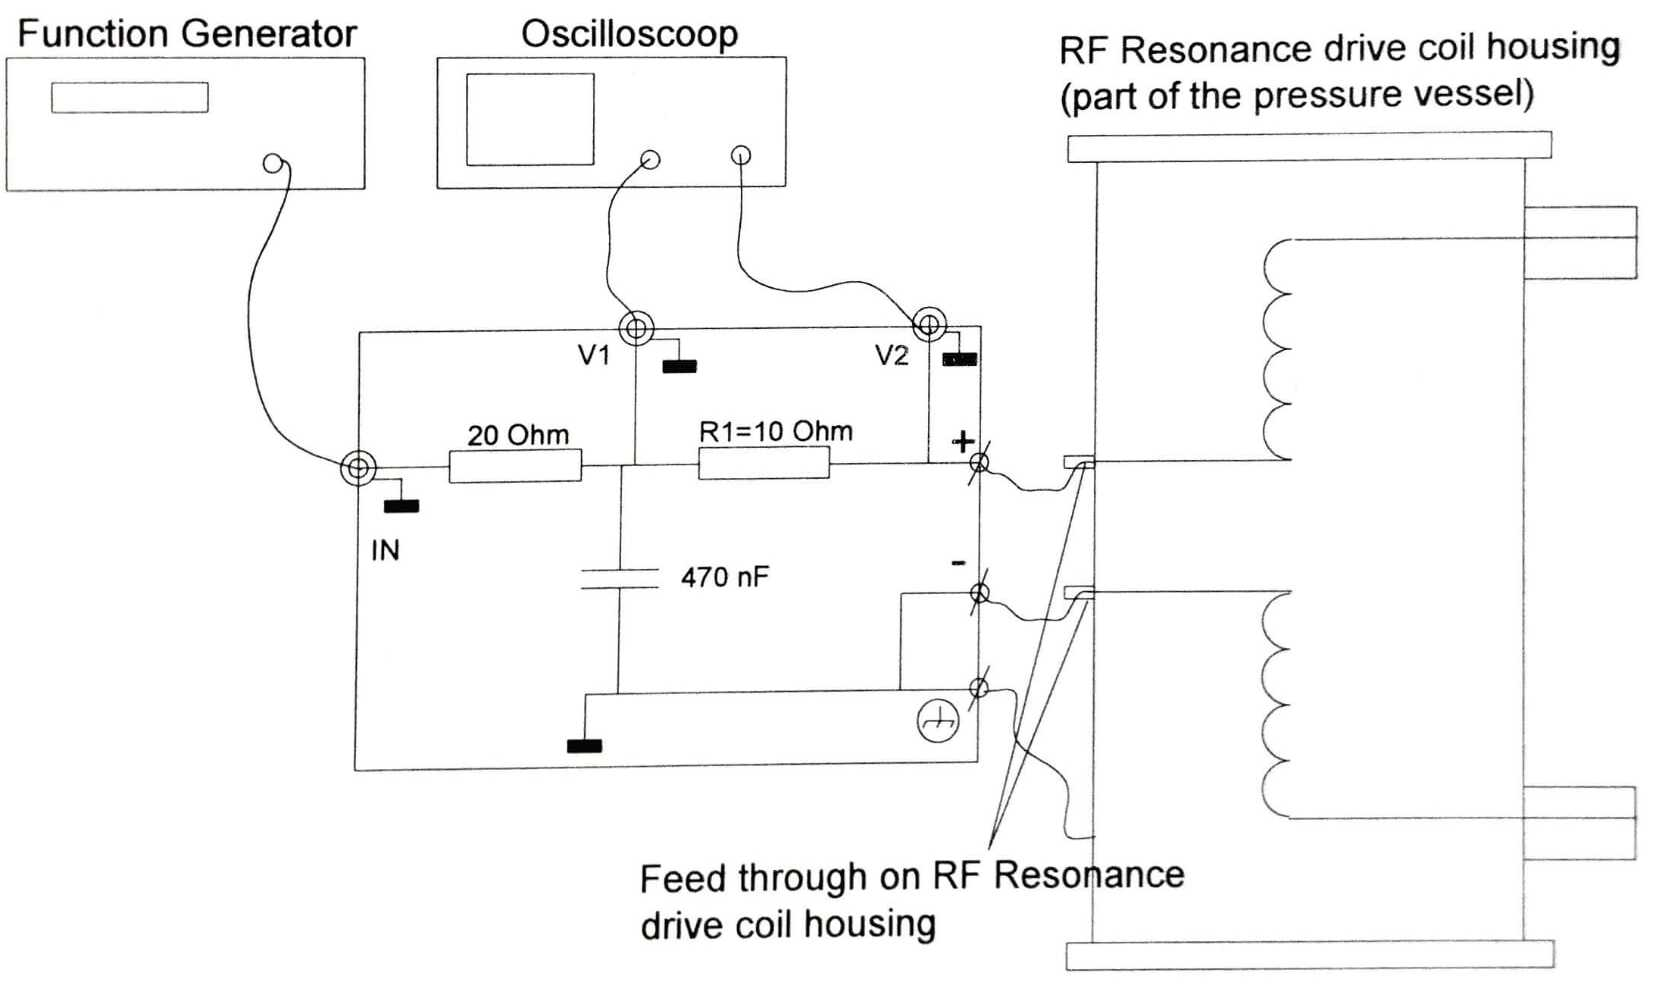
\includegraphics[width=0.49\textwidth]{Figures/MEG/CW/cw_qfactor.jpeg}\label{fig:CW:sketch:Q-factor}}
            \hfill
            \subfloat[Example of measurement of the Q-factor: in red the delay while in blue the fraction $V_1/V_2$.]{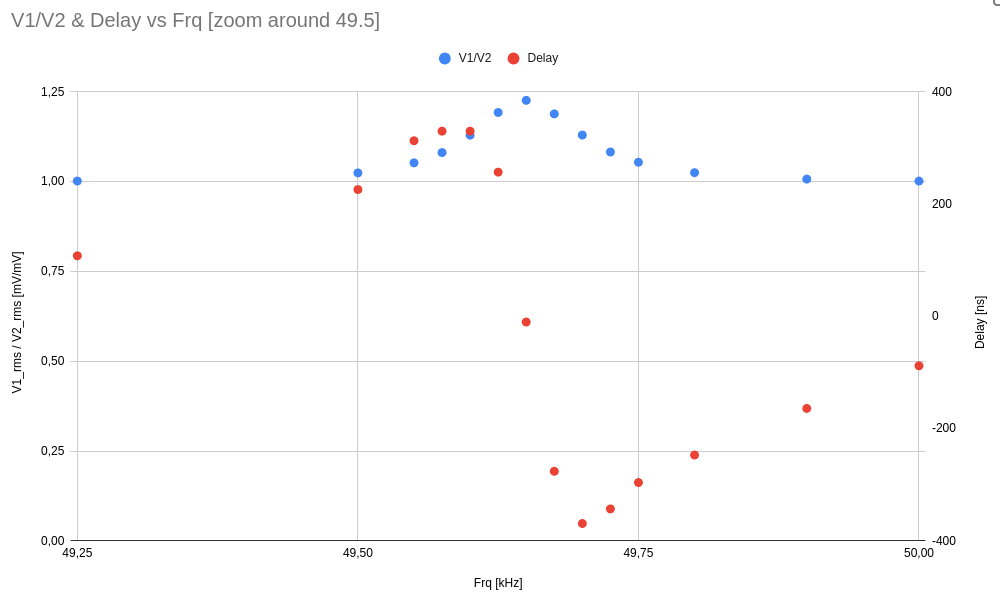
\includegraphics[width=0.49\textwidth]{Figures/MEG/CW/CW_Q-factor.png}\label{fig:CW:Q-factor}}
            \caption{The Q-factor is the ratio of blind to dissipated power. Via this number is possible to evaluate the energy dissipated as heat running the machine. If it is too low the machine cannot operate correctly.}
        \end{figure}

        \begin{figure}
            \centering
            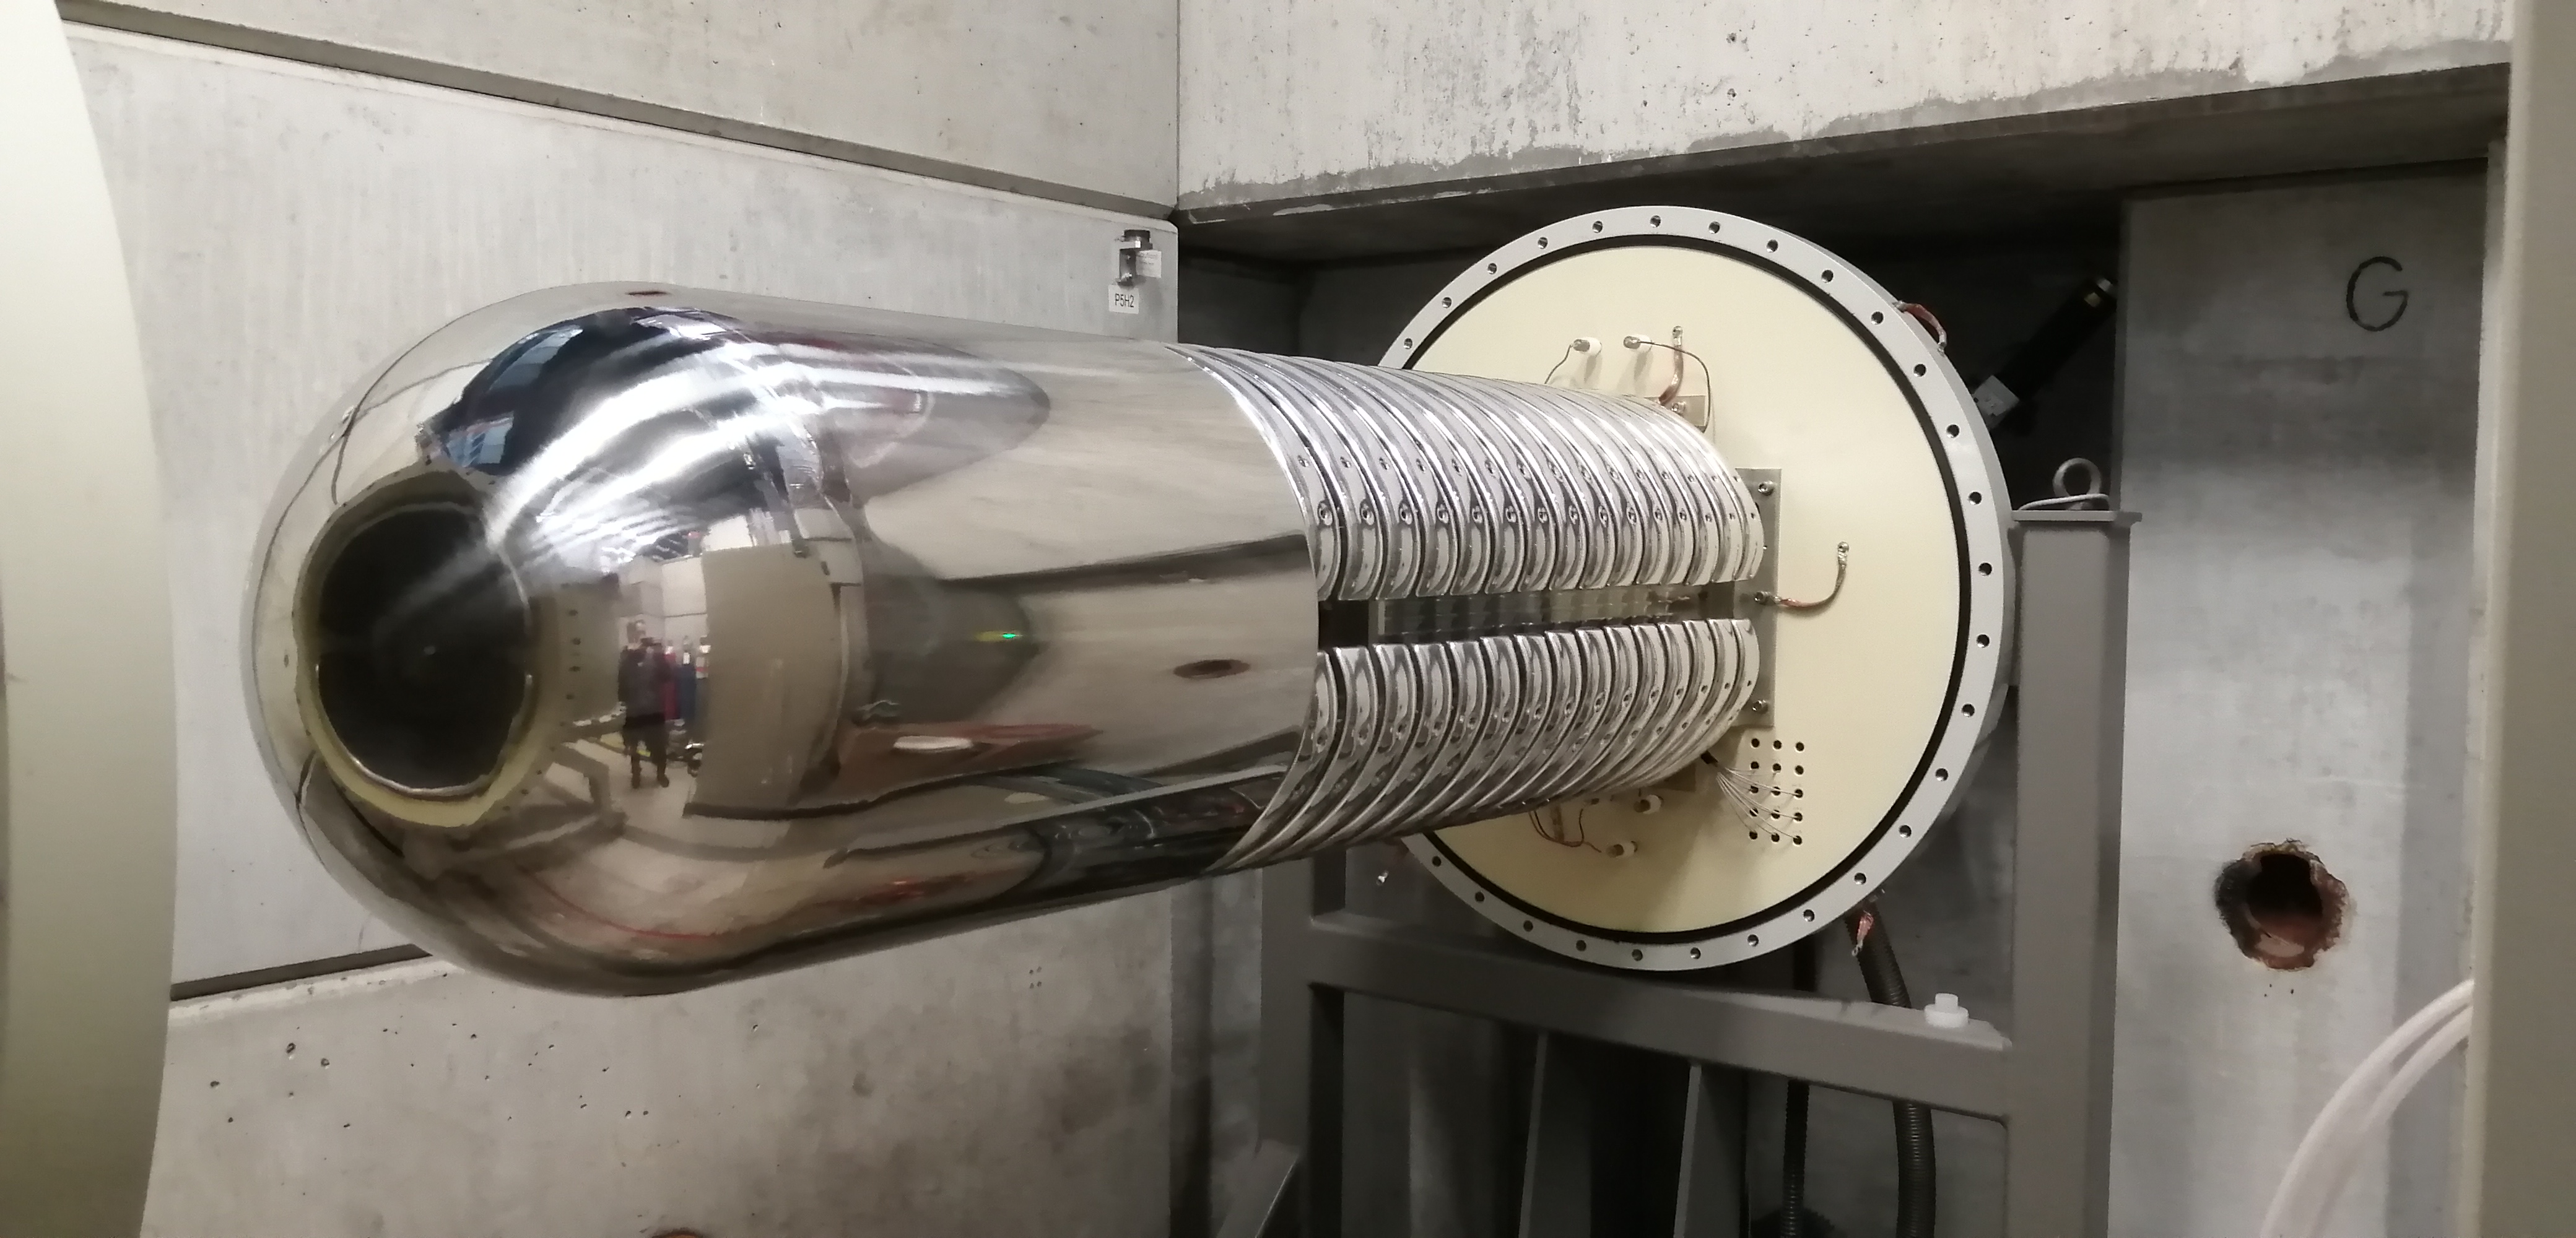
\includegraphics[width=1\textwidth]{Figures/MEG/CW/view_front.jpg}
            \caption{View of the CW after the extraction from the external volume. This volume contains \ce{SF6} which is used as a gaseous dielectric medium and needs to be evacuated before the extraction.}
            \label{fig:CW:view}
        \end{figure}

        \begin{figure}
            \centering
            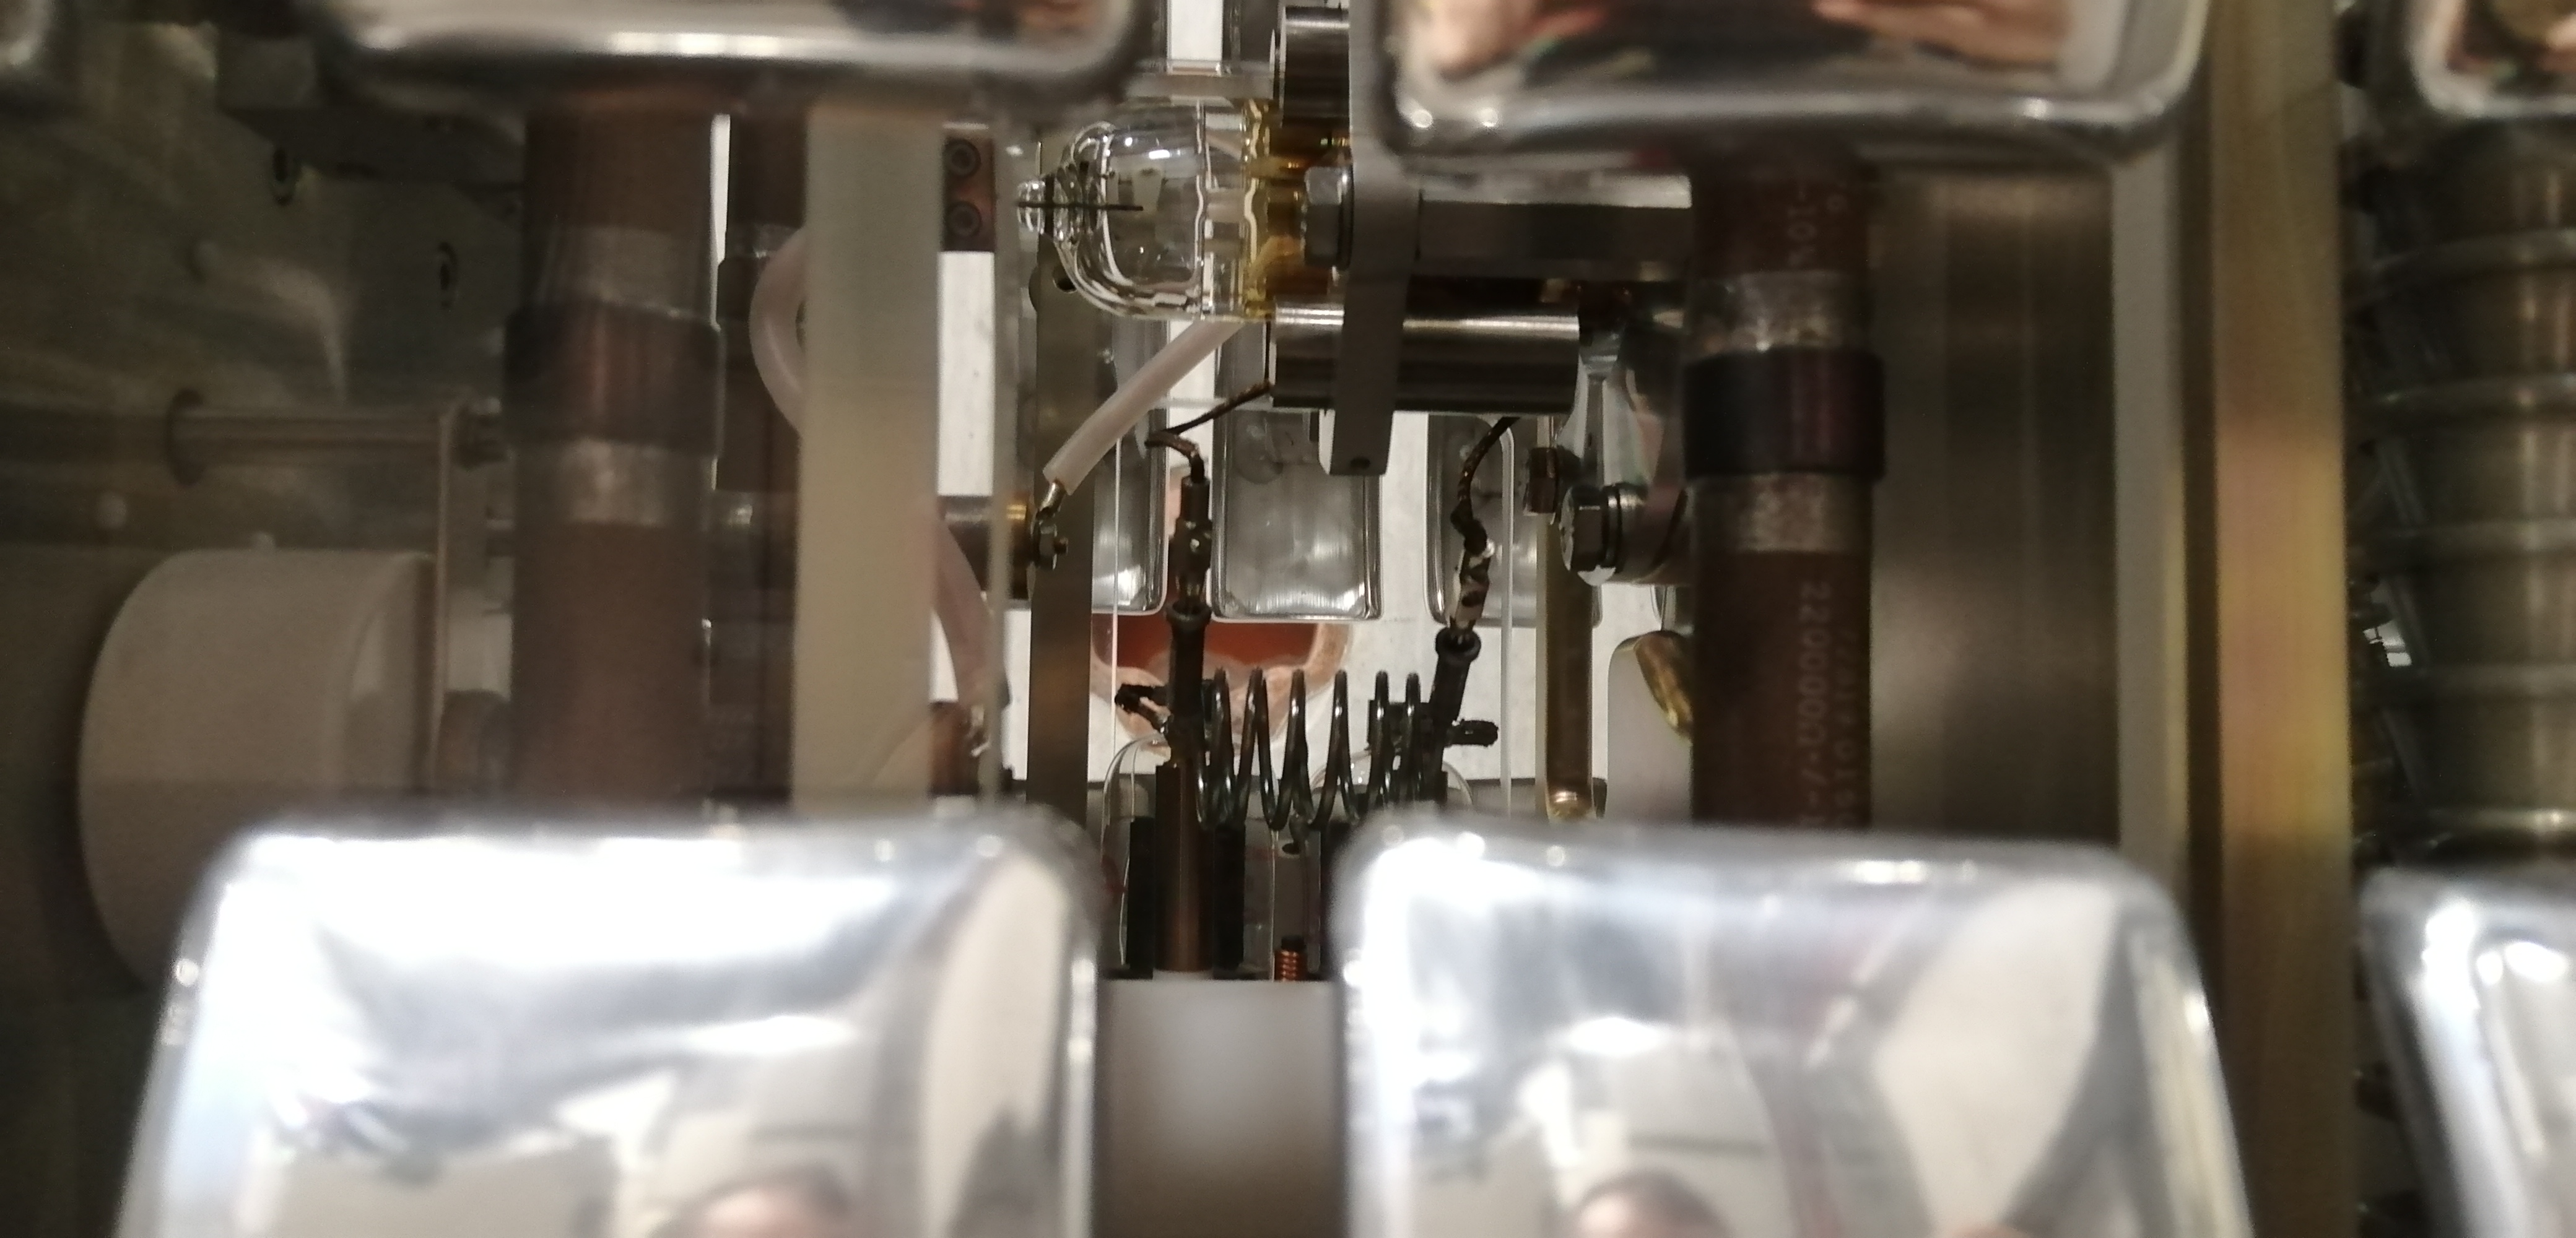
\includegraphics[width=1\textwidth]{Figures/MEG/CW/view_source.jpg}
            \caption{View of the source of the CW   machine.}
            \label{fig:CW:view_source}
        \end{figure}

        \begin{figure}
            \centering
            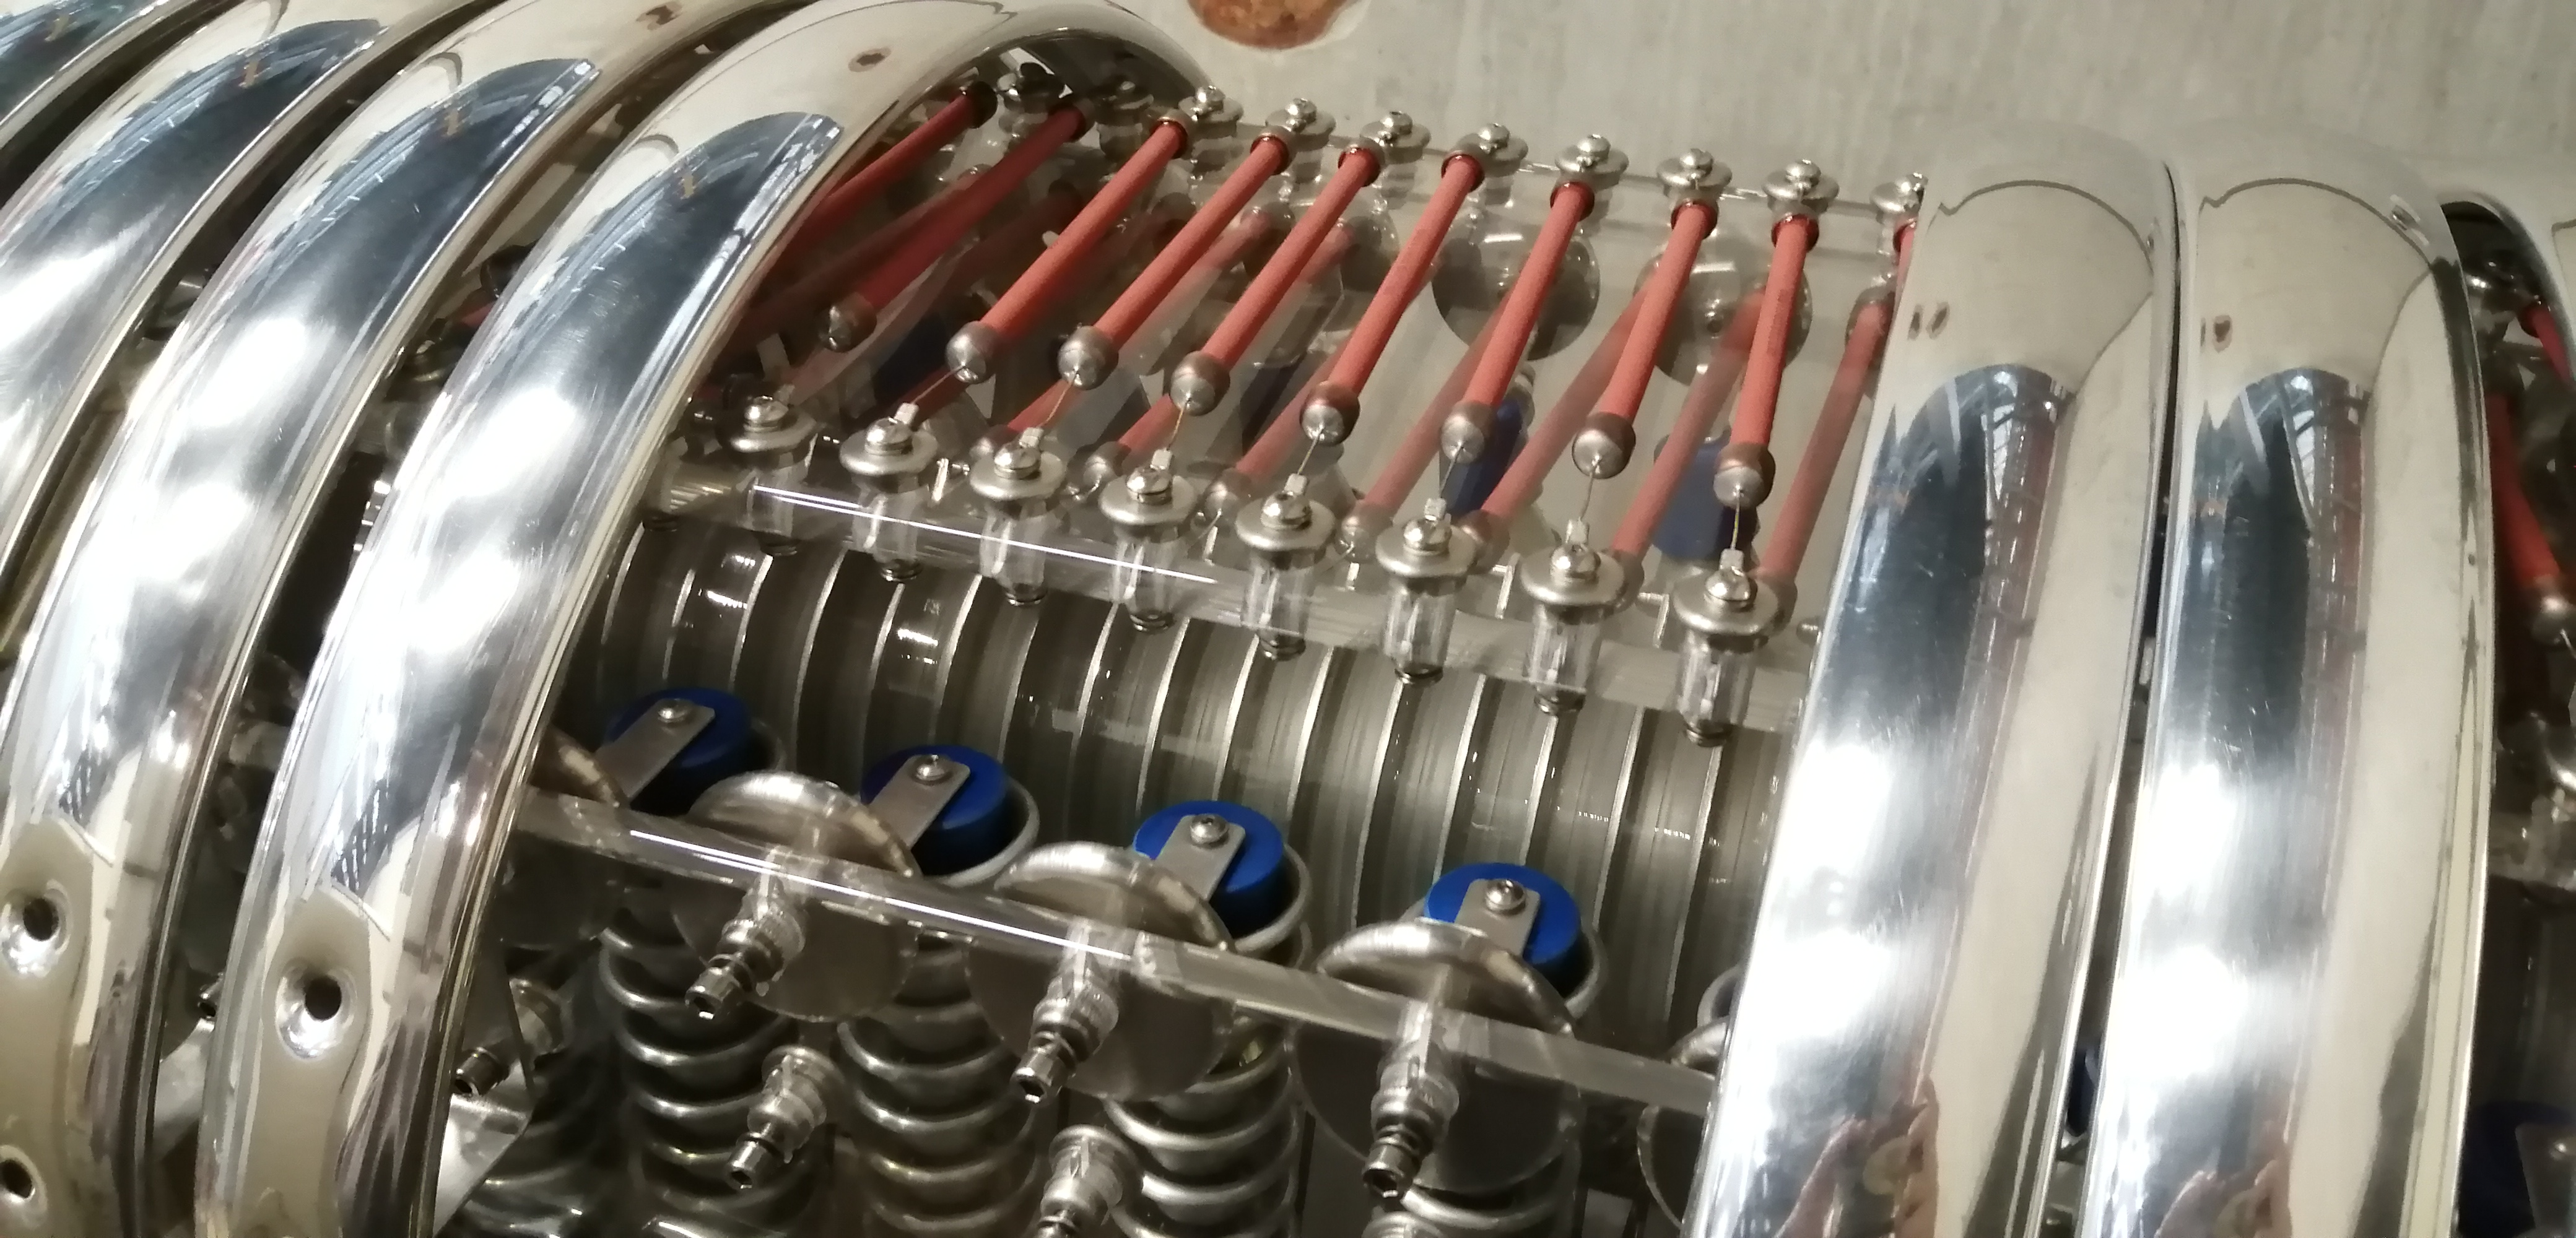
\includegraphics[width=1\textwidth]{Figures/MEG/CW/view_top.jpg}
            \caption{Top view of the CW after the removal of a few \textit{corona rings}. Here we can see all the elements of a CW circuit: red - the resistors on top; metallic rings on the central tube - the capacitors; blue and metallic cups - the resistance and capacitors of the rectifiers, which run vertically.}
            \label{fig:CW:view_top}
        \end{figure}

        \begin{figure}
            \centering
            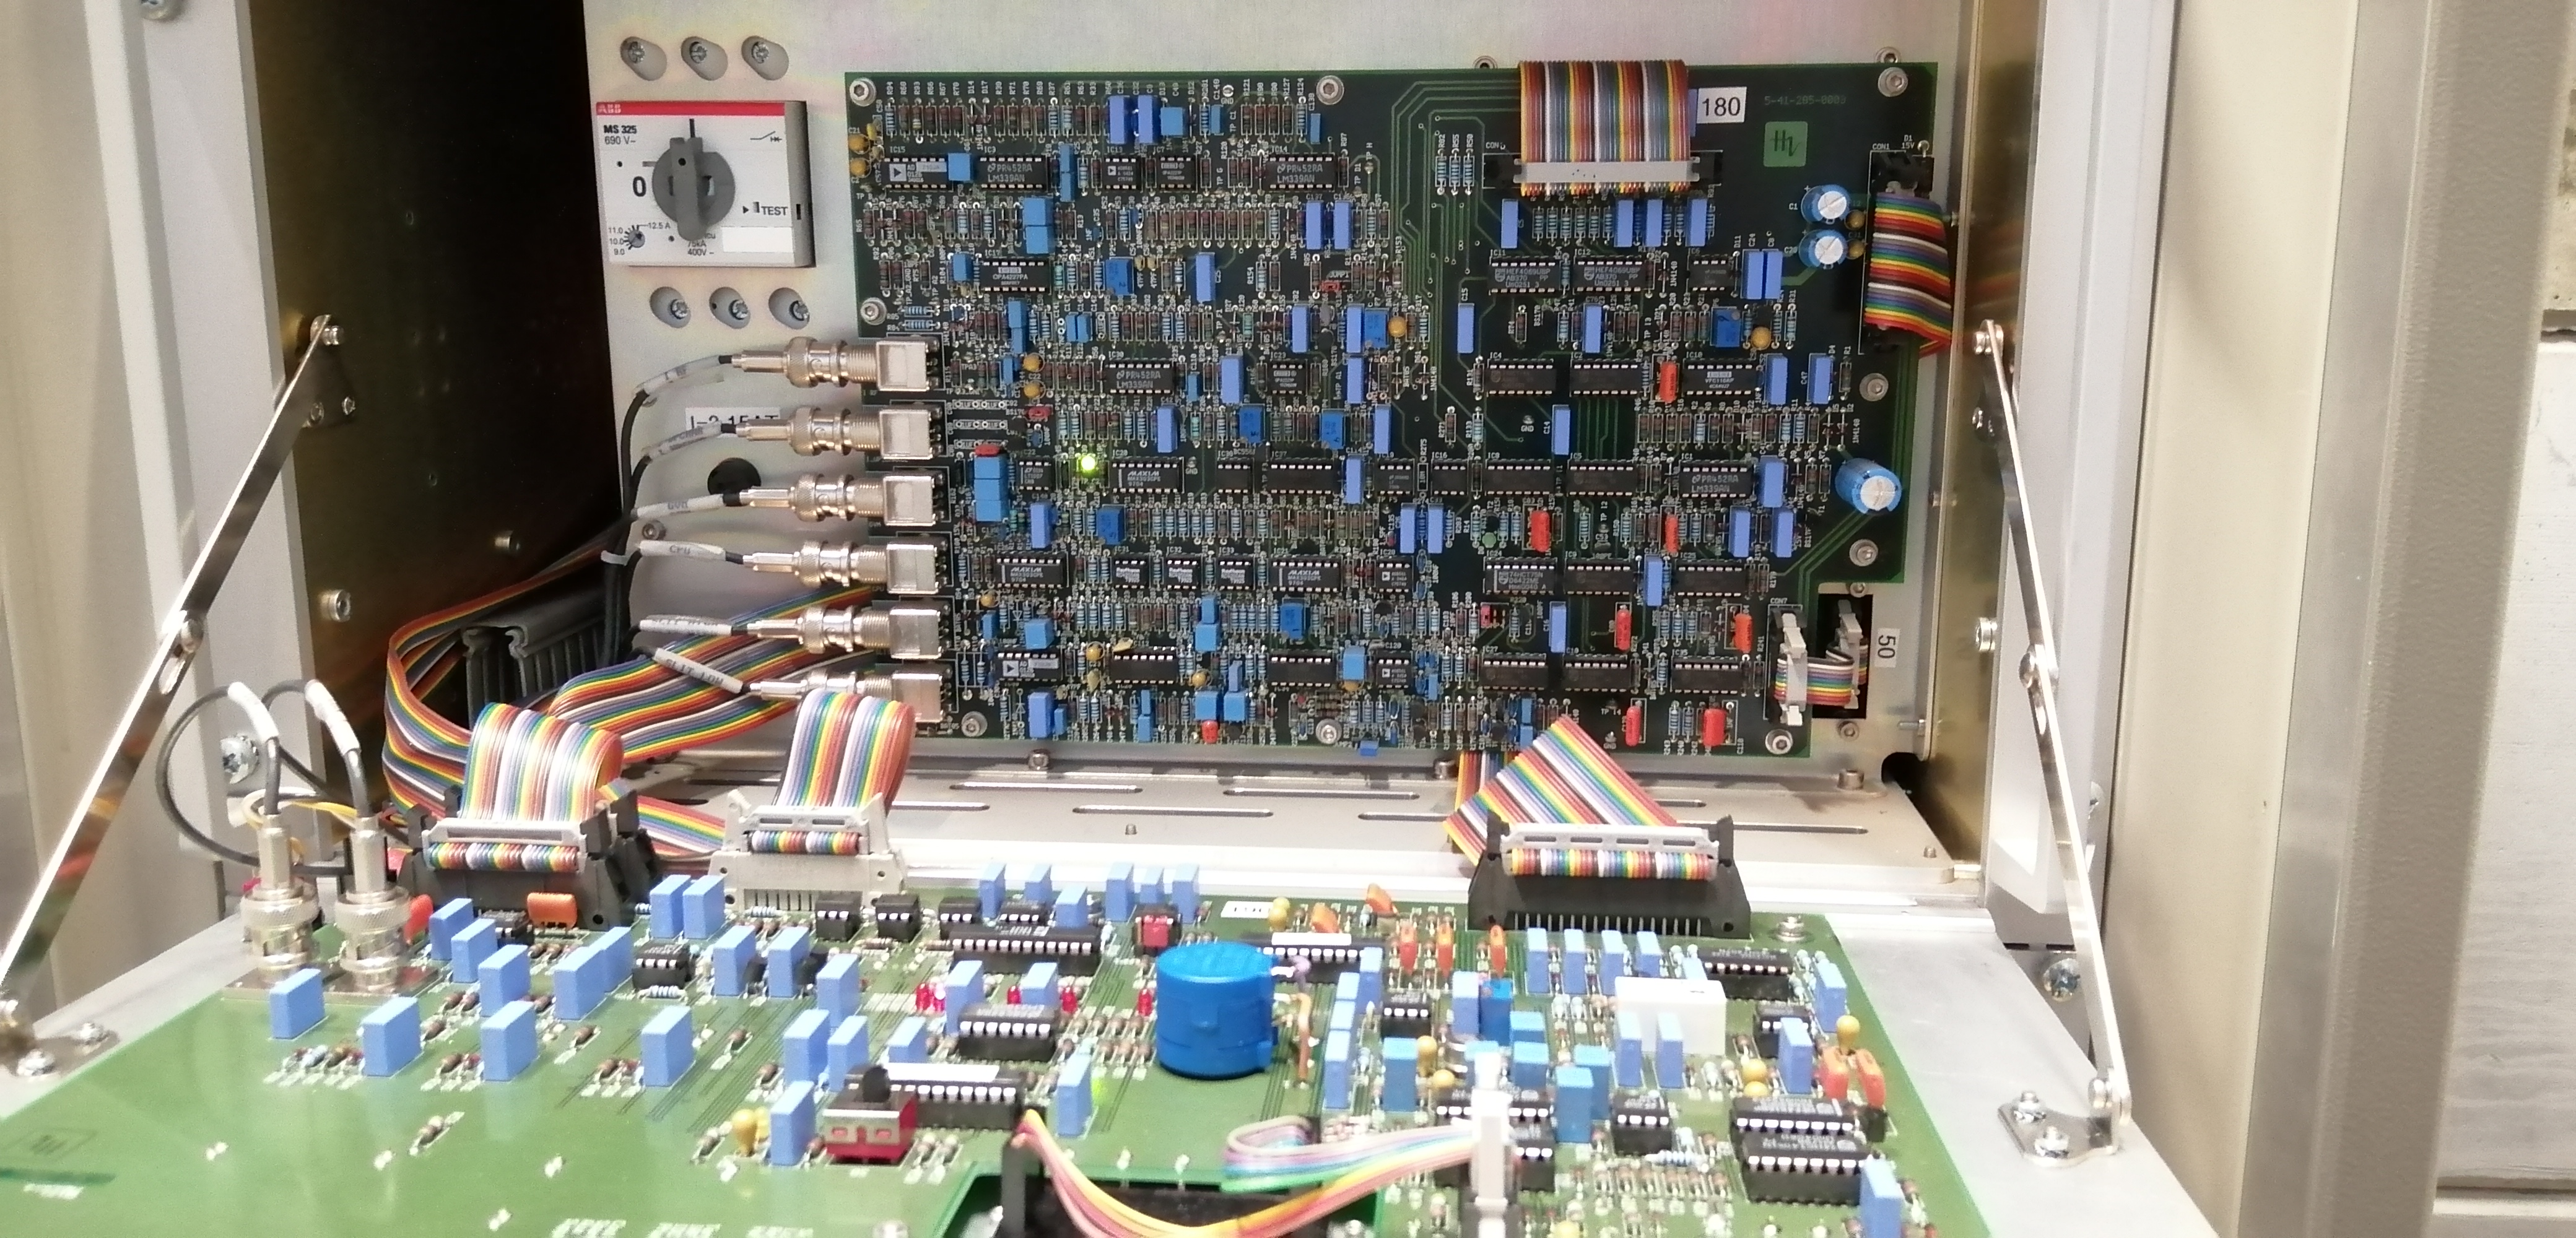
\includegraphics[width=1\textwidth]{Figures/MEG/CW/panel.jpg}
            \caption{Picture of the control panel for the CW machine.}
            \label{fig:CW:panel}
        \end{figure}

    \status{review}
    \subsection{Usage}
        This machine is used 3 times a week, together with a \ce{^7Li} target, to produce the \SI{17.6}{MeV} line of the \ce{^7Li(p,\g)^8Be} to calibrate the XEC. 
        This process was already outlined in Sec.~\ref{sec:MEG:XEC:calibrations}.
        On top of taking care of these calibrations\footnote{This 3 times a week task was shared between 3 people, me included.} I ironed out the procedure and reworked the documentation.
        
        \paragraph{X17} The protons coming from the CW have been mainly used for the calibration of the XEC detector, but also to perform a parasitic measurement:the search for the X17 anomaly.
        This search, done in 2021-2023, will be extensively discussed in Ch.~\ref{ch:X17} but we wanted to underline here the key role that the CW machine has played in this parasitic search for exotic physics. 

    \status{review}
    \subsection{CW issues and maintenance}
        By the end of 2020, the CW started having some minor problems: the machine was running fine but the time required to switch it on kept growing longer. 
        While the whole procedure would normally take $\sim$ 15 min the time required exceeded the hour.
        We also noticed the machine was getting unstable when running near the maximum voltage at \SI{1}{MV}.
        Following this behavior, an intense exchange with the HVEE company started and we performed many different tests on both the software and hardware sides.
    
        \paragraph{Hot Fix}
        We performed a measurement of the Q-factor of the machine using Eq.~\ref{eq:cw:qfactor}, shown in Fig. \ref{fig:CW:Q-factor}.  
        The value found was a factor $\sim2k$ lower than expected and the position of the resonance frequency was shifted from the design value.
        For more information on the functioning of the machine and the Q-factor see Sec.~\ref{sec:cw:machine}.
        We adjusted the frequency at which the machine starts when turning ON. 
        This solved the delay problem but didn't recover the maximum voltage. \\
        The machine was now starting quickly but working in a stable configuration only up to half of the nominal maximum voltage.
        As explained in the previous paragraph this was not a problem for the `usual' calibrations but was a worrying sign on the health of the machine and would have prevented the CEX.
        At this point, an expert from HVEE was sent to inspect the machine.

        \paragraph{Maintenance}
        After running some checks opening the CW was deemed necessary and for this reason, we removed the \ce{SF6} contained in the main tank. 
        After the extraction of the CW, we inspected and measured all the elements, removing also some of the \textit{corona rings} for easier inspection. 
        We found signs of arcing on one of the \textit{rectifier ass'y}. 
        After the substitution of this element\footnote{The rectifier ass'y are stacks of alternated diodes and aluminum capacitors capped by two resistors. We could re-use the capacitors, after careful cleaning, while resistors and diodes were too badly damaged. The process of refurbishing is shown in Fig.~\ref{fig:CW:fixed}}, the machine was closed again, filled with \ce{SF6}, and tested again.
        This whole process is shown in the pictures in Fig.~\ref{fig:CW:broken}.
        Unfortunately, the faulty behavior persisted and we noticed sparks in the main volume. 
        After re-opening we found burning marks on the rectifier ass'y next to the exchanged one.
        We then realized that both were damaged but the first was functioning as a `bridge', preventing the second from being completely destroyed. 
        After the substitution of the second and the tuning of the machine, we finally recovered its full functionality: quick switching ON and stable operation in the full range of voltages.
        \ref{fig:CW:fixed}.

        \begin{figure}[ht]   
            \centering
            \subfloat[Discovery of the burning marks on two rectifiers. The reflectivity was a challenge in taking the picture.]{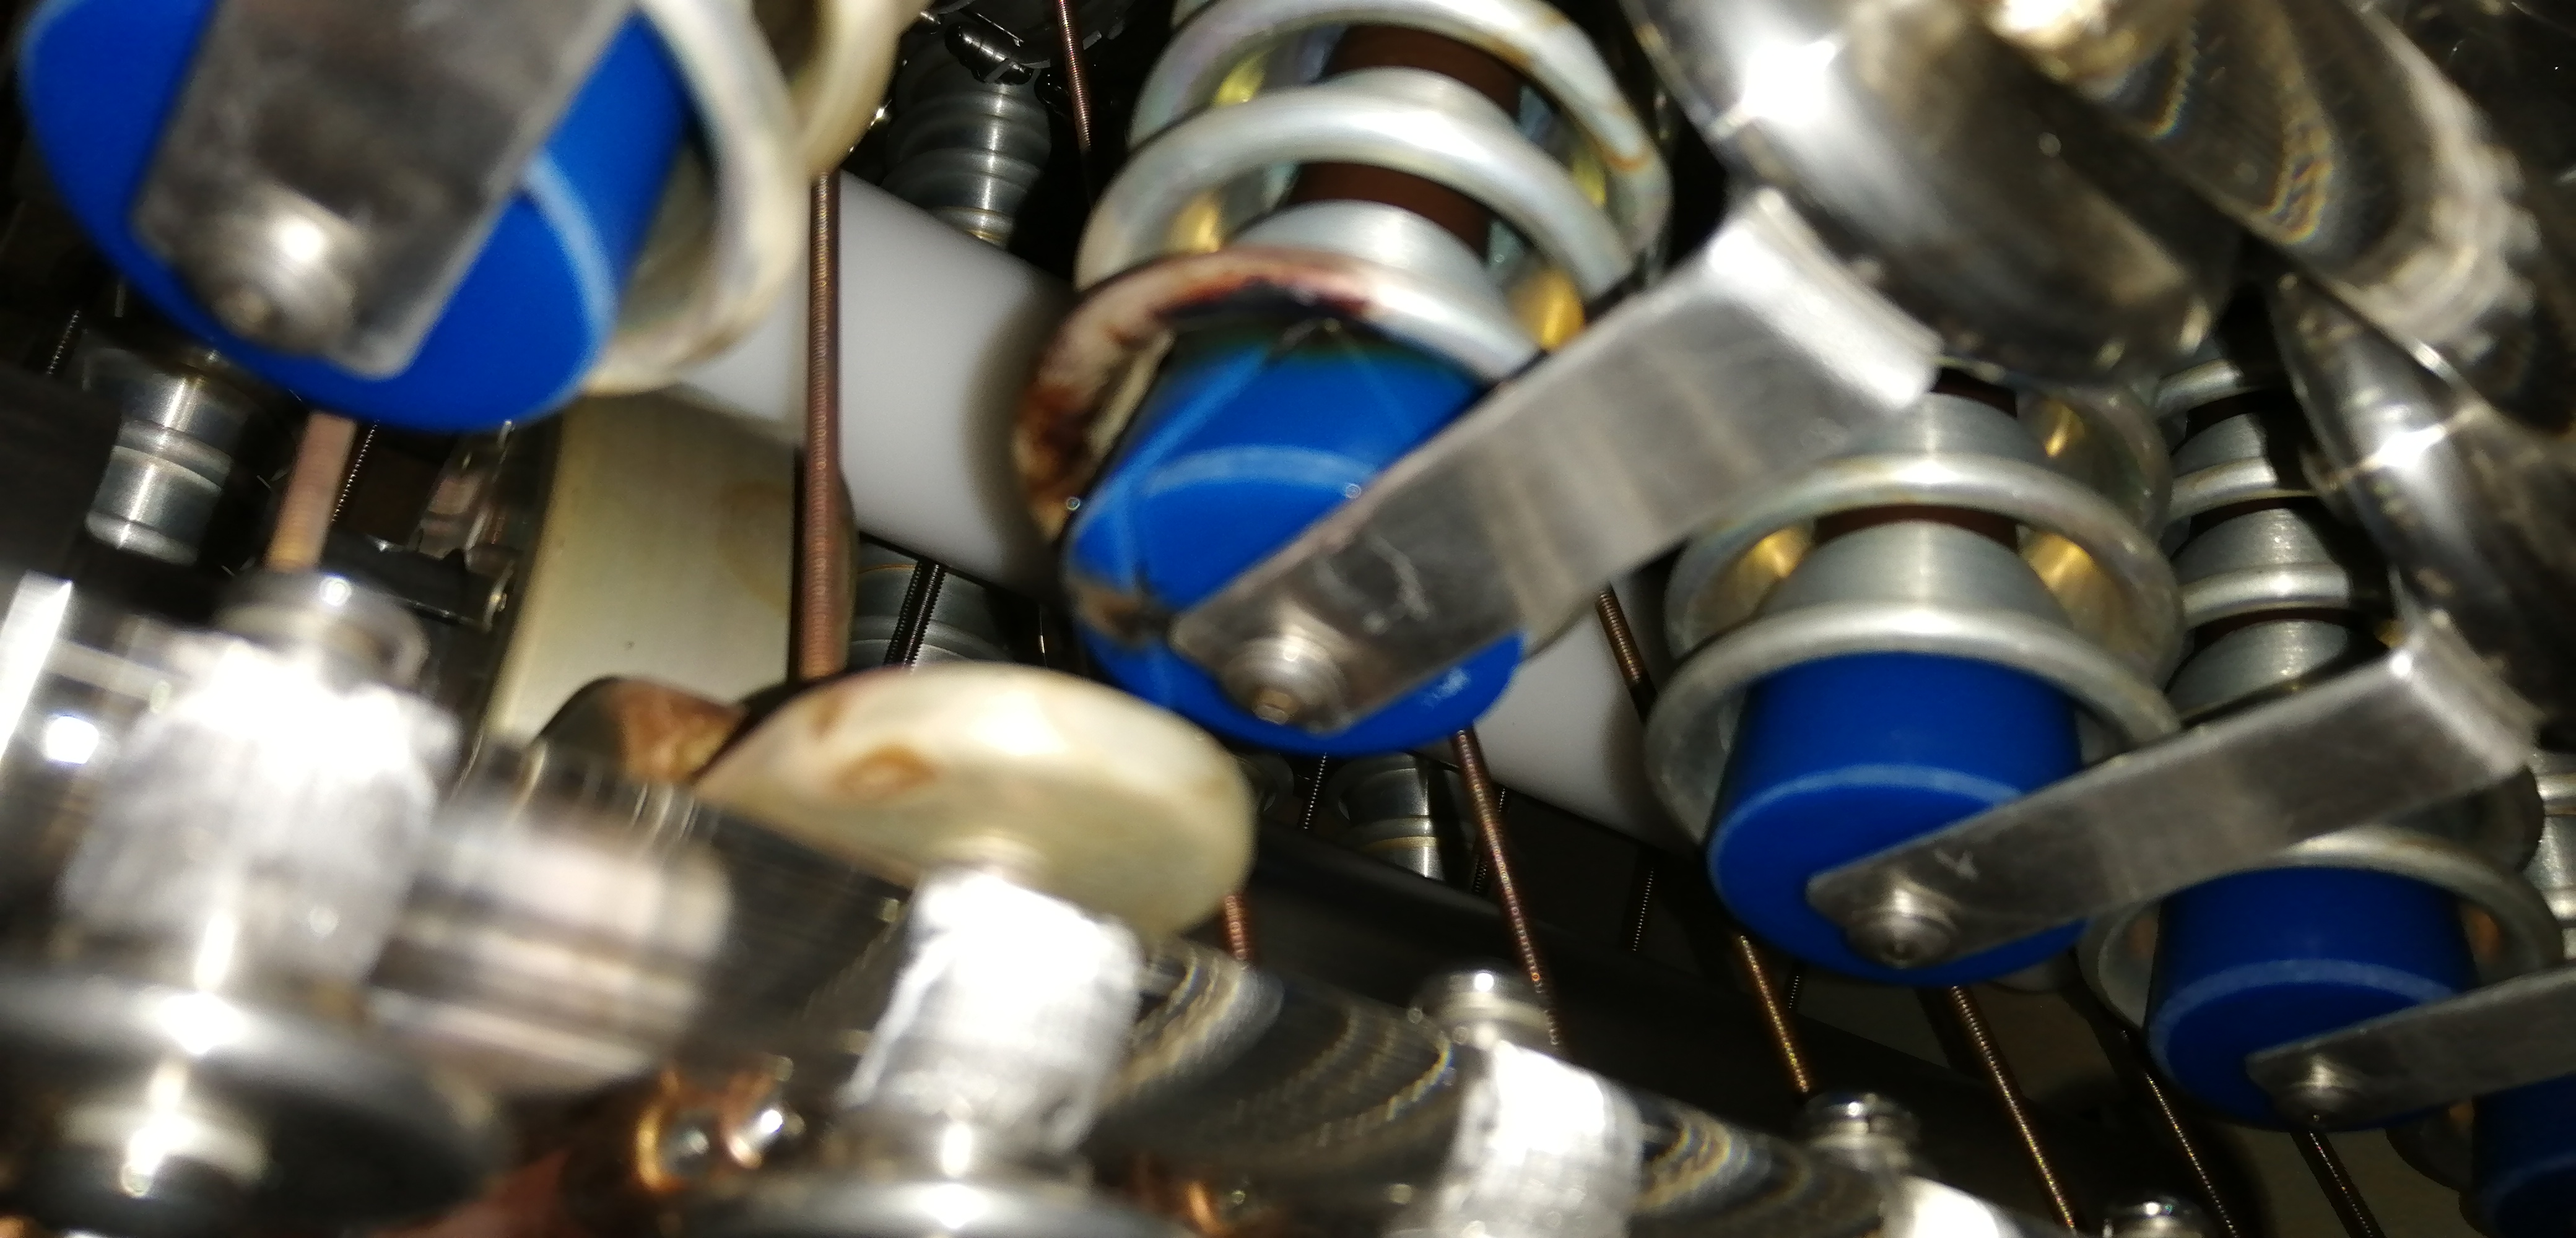
\includegraphics[width=1\textwidth, keepaspectratio]{Figures/MEG/CW/bnurned_in.jpg}\label{fig:CW:burned_in}}\\
            \subfloat[Extraction of the broken rectifiers.]{
            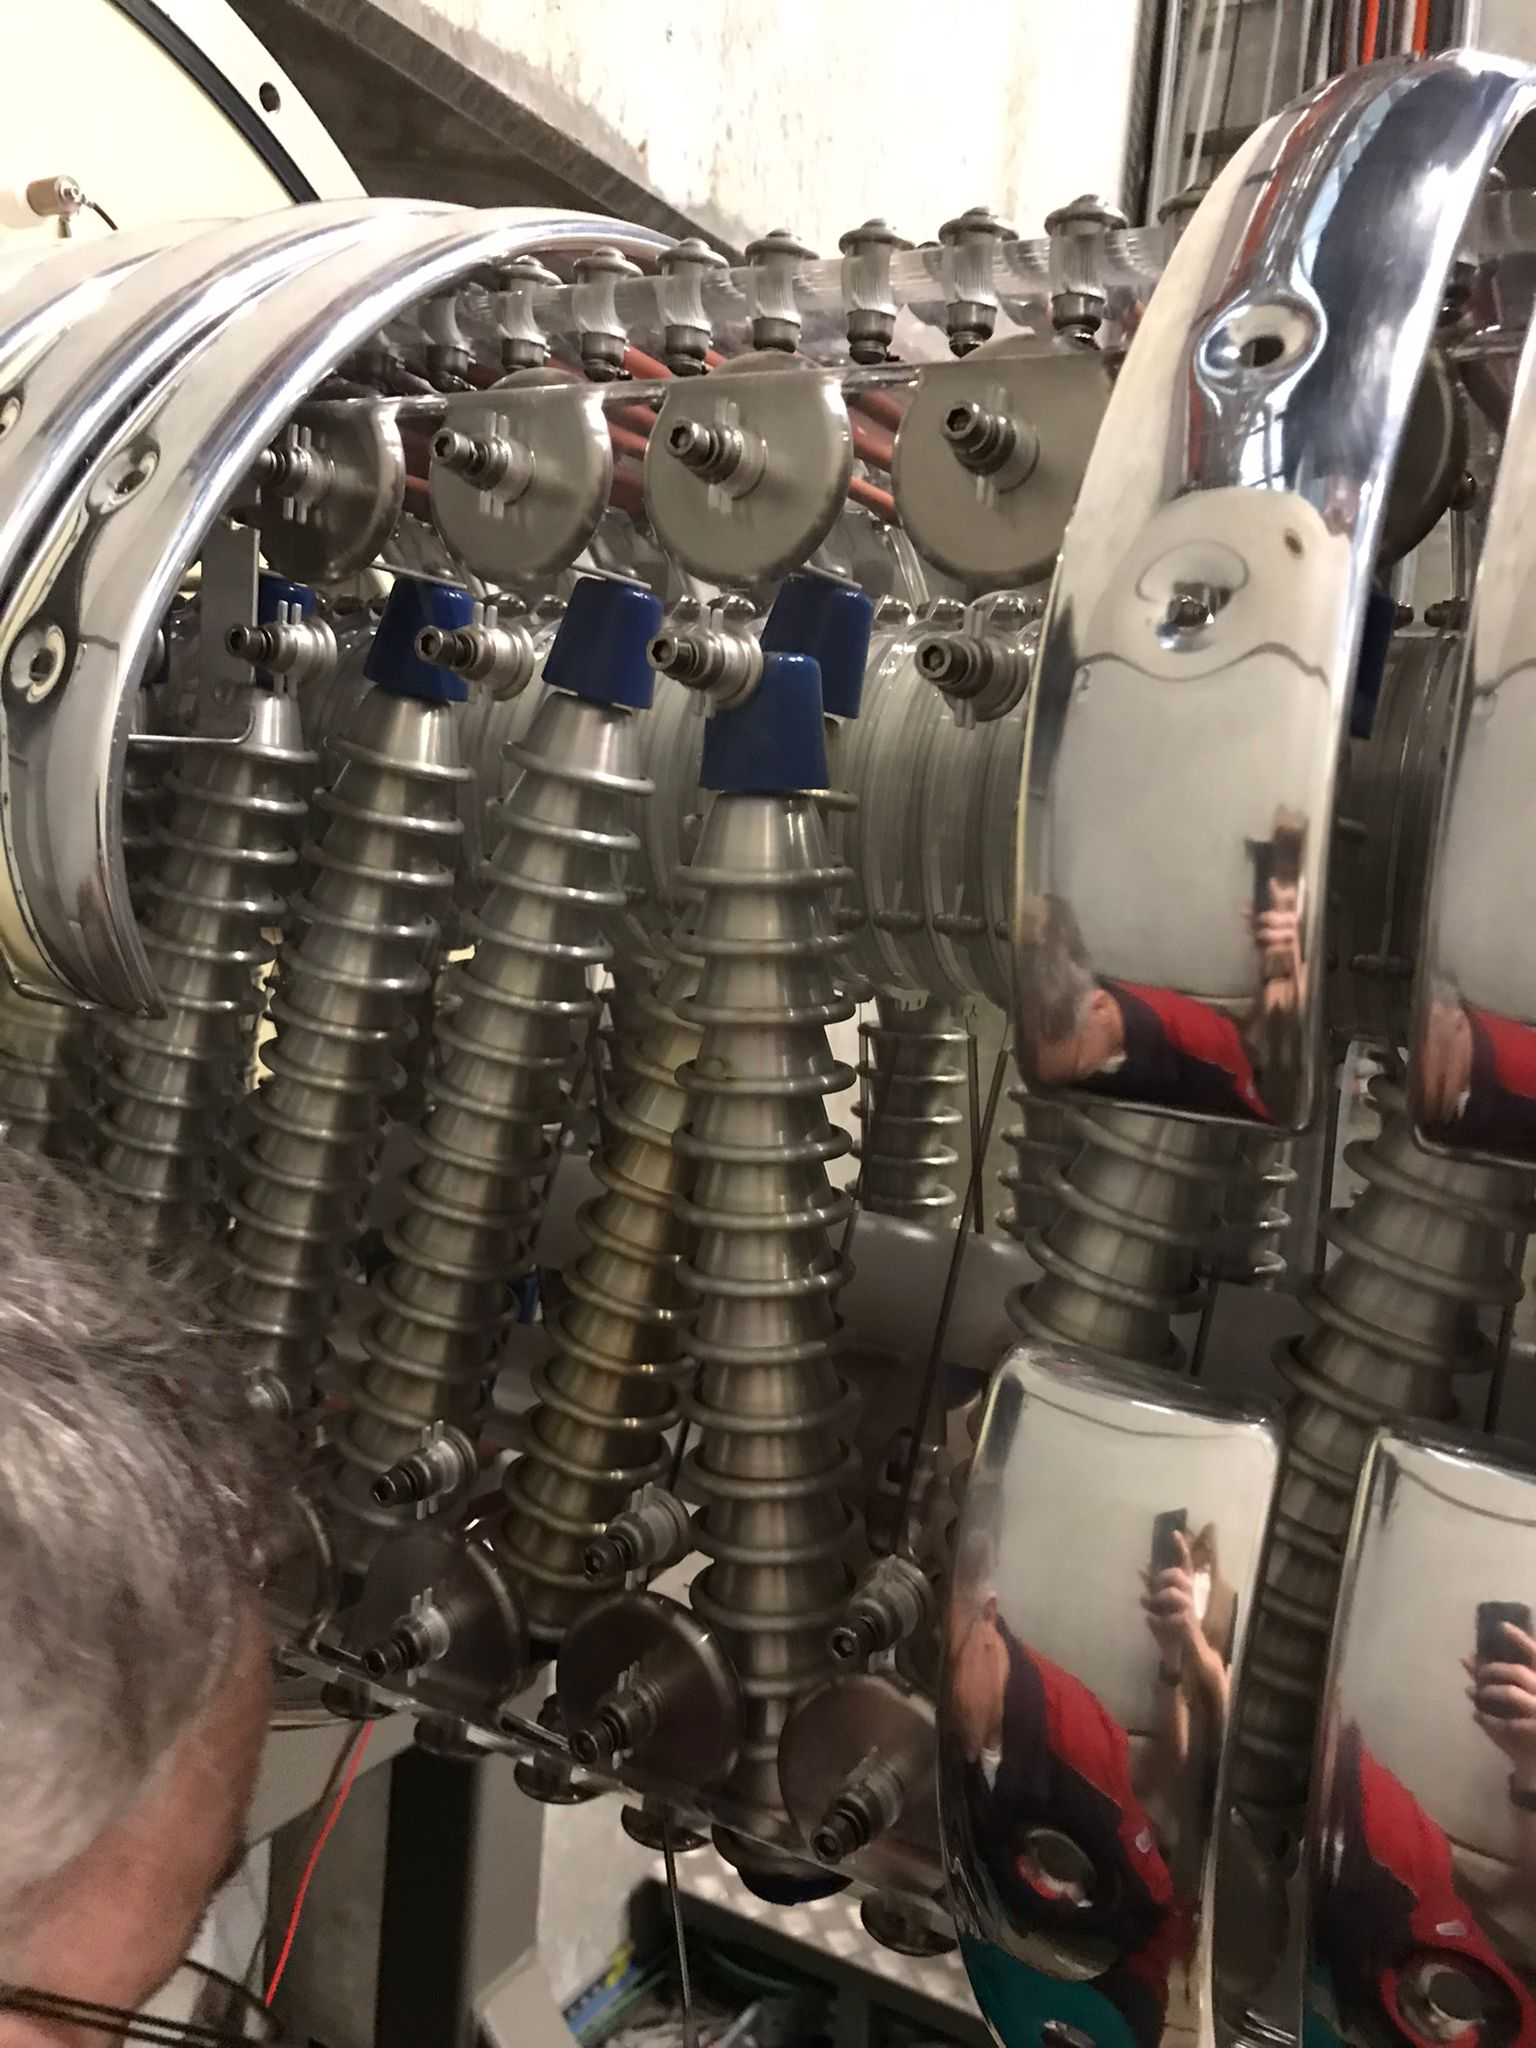
\includegraphics[width=0.49\textwidth, keepaspectratio]{Figures/MEG/CW/removal.jpg}\label{fig:CW:removal}}
            \hfill
            \subfloat[Broken rectifier ass'y after the extraction: clearly visible is the burned blue resistor at the top.]{
            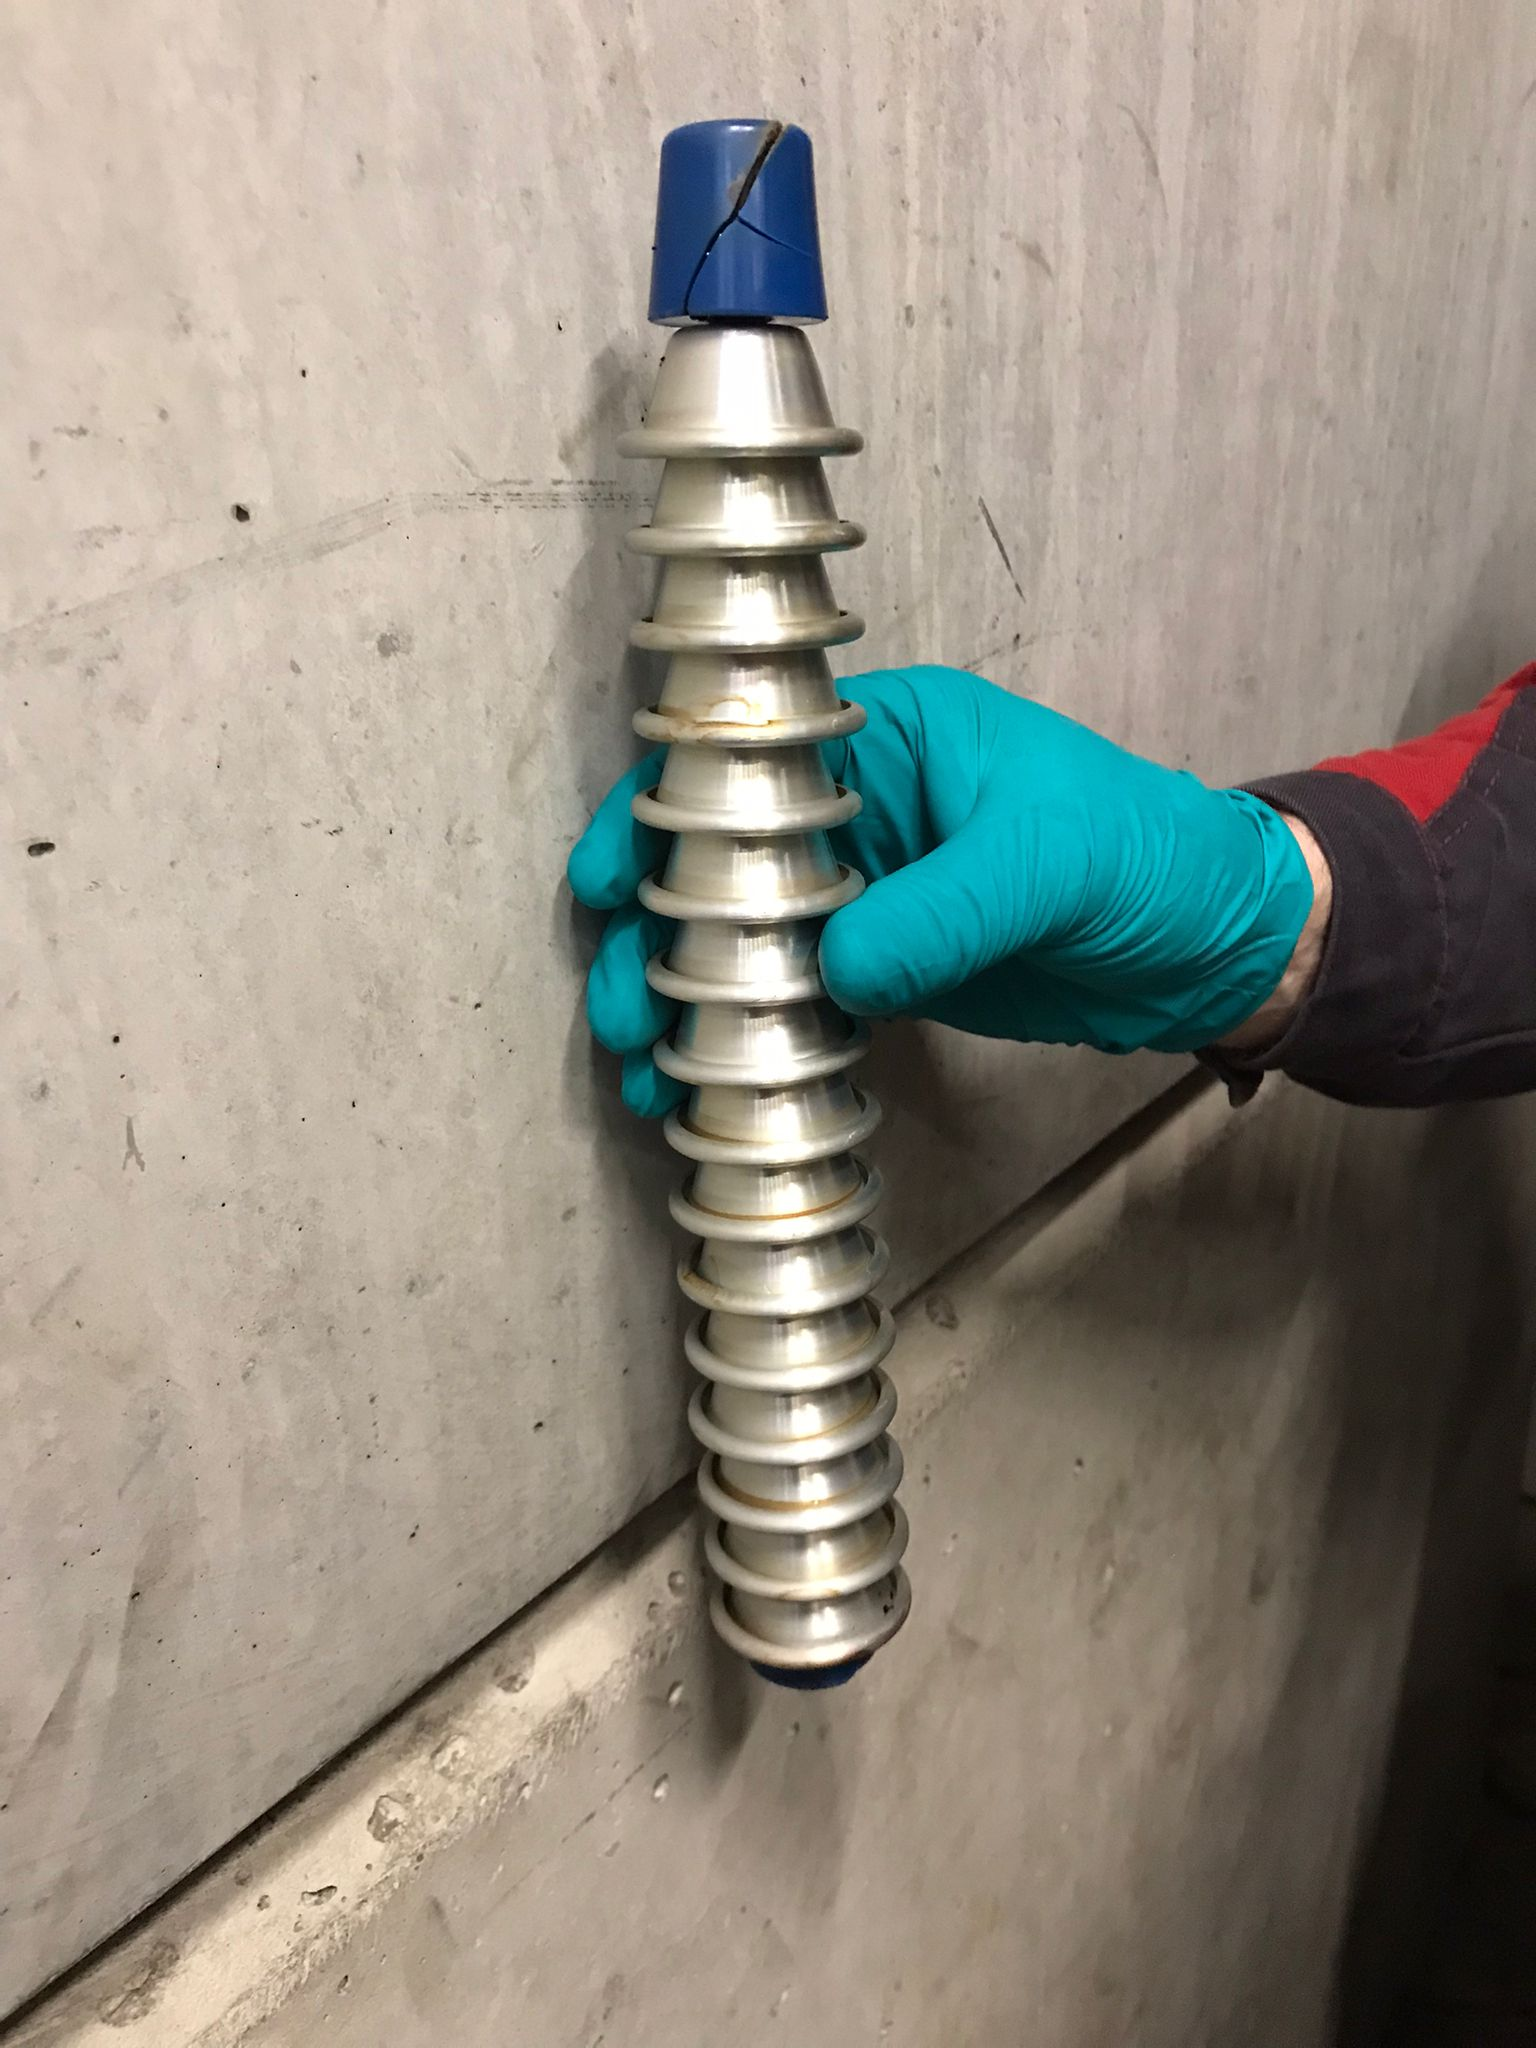
\includegraphics[width=0.49\textwidth, keepaspectratio]{Figures/MEG/CW/rect_broken.jpg}\label{fig:CW:rect_broken}}
            \caption{After close inspection we found burning marks on two rectifiers' ass'y (\ref{fig:CW:burned_in}). These were removed (\ref{fig:CW:removal}) and carefully inspected (\ref{fig:CW:rect_broken}). The only salvageable part of the rectifiers were the aluminum capacitors, which we cleaned from burning residuals, while all diodes and resistors had to be exchanged.}
            \label{fig:CW:broken}
        \end{figure}

        \begin{figure}[ht]   
            \centering
            \subfloat[Picture of the burning marks on the end resistors of the rectifier ass'y.]{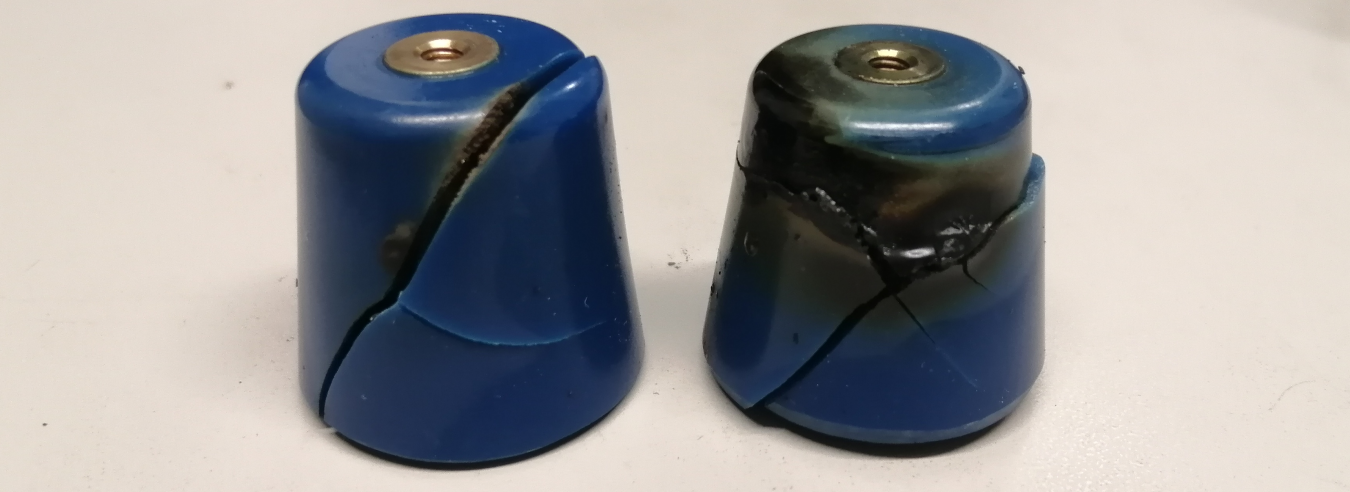
\includegraphics[width=1\textwidth, keepaspectratio]{Figures/MEG/CW/burned.png}\label{fig:CW:burned}}\\
            \subfloat[Assembly of one of the new stack: black - resistors; brown - diodes; metallic - aluminum capacitors.]{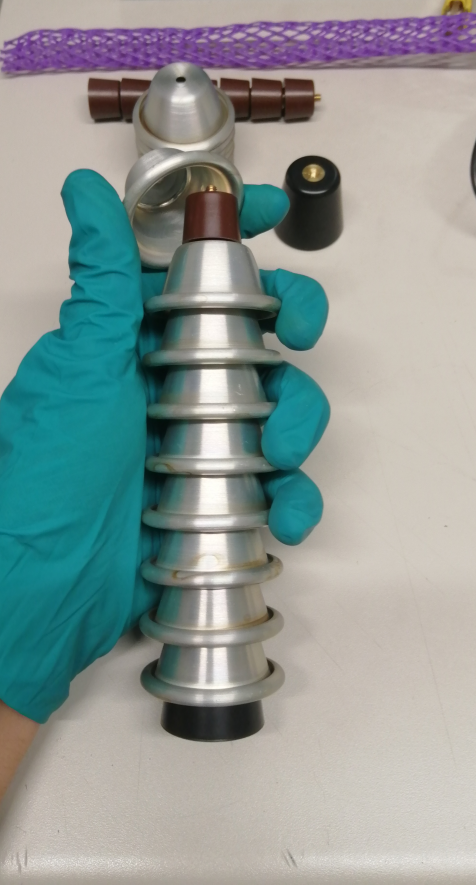
\includegraphics[width=0.49\textwidth]{Figures/MEG/CW/rect_build.png}\label{fig:CW:rect_build}}
            \hfill
            \subfloat[One of the finished new rectifiers.]{       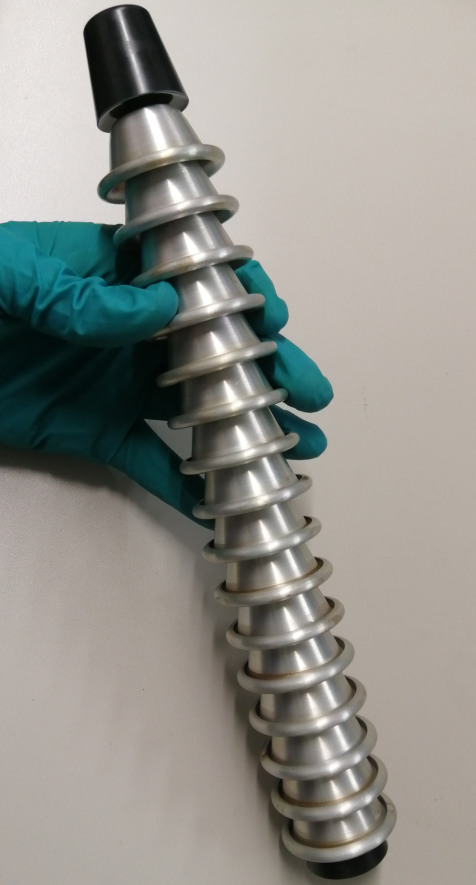
\includegraphics[width=0.49\textwidth, keepaspectratio]{Figures/MEG/CW/rect_new.png}\label{fig:CW:rect_new}}
            \caption{The rectifiers are made of three elements: diodes; aluminum capacitors; resistors (\ref{fig:CW:burned}). Only the capacitors were salvageable: we re-assembled the rectifiers with new diodes and resistors (\ref{fig:CW:rect_build}; \ref{fig:CW:rect_new}).}
            \label{fig:CW:fixed}
        \end{figure}

\status{review}
\section{Conclusions}
In this (very dense) chapter we went through the description of two key elements of the work I have done during these three years: the MEG II apparatus and the Cockcroft–Walton.
While I took no part in the design of either, in these years I spent a lot of time `hands-on' on many subsystems of the MEG II apparatus: calibrations, tuning, and fixes of various types.
On the other side, the CW functioning has been one of my main tasks.
The unfortunate hiccup with it gave me the additional unforeseen opportunity to assist the HVEE technician in testing and fixing the machine, which was an extremely interesting and instructive experience. 

\status{started}
\printbibliography[
    heading = bibliographychapter,
    title=Bibliography on MEG II
]

\end{refsection}
